%%%%%%%%%%%%%%%%%%%%%%%%%%%%%%%%%%%%%%%%%

%----------------------------------------------------------------------------------------
%	PACKAGES AND OTHER DOCUMENT CONFIGURATIONS
%----------------------------------------------------------------------------------------

\documentclass[
12pt, % The default document font size, options: 10pt, 11pt, 12pt
%oneside, % Two side (alternating margins) for binding by default, uncomment to switch to one side
french, %english, % ngerman for German
 % singlespacing, % Single line spacing, alternatives: onehalfspacing or doublespacing
%draft, % Uncomment to enable draft mode (no pictures, no links, overfull hboxes indicated)
%nolistspacing, % If the document is onehalfspacing or doublespacing, uncomment this to set spacing in lists to single
%liststotoc, % Uncomment to add the list of figures/tables/etc to the table of contents
toctotoc, % Uncomment to add the main table of contents to the table of contents
%parskip, % Uncomment to add space between paragraphs
%nohyperref, % Uncomment to not load the hyperref package
headsepline, % Uncomment to get a line under the header
%chapterinoneline, % Uncomment to place the chapter title next to the number on one line
%consistentlayout, % Uncomment to change the layout of the declaration, abstract and acknowledgements pages to match the default layout
]{MastersDoctoralThesis} % The class file specifying the document structure

%Options : inlinechap, quotchpI, boxedchapnum, boxedchapnumN, quotchapII, roundchapnum, boxedchapnumL, boxedchapnumR
\usepackage[boxedchapnum]{settings/fncystyle}
\usepackage[sloped]{fourier}
\usepackage[utf8]{inputenc} % Required for inputting international characters
\usepackage[T1]{fontenc} % Output font encoding for international characters
\usepackage{verbatim}
\usepackage{mathpazo} % Use the Palatino font by default
\usepackage{enumitem}
\usepackage{amssymb,amsmath}
\usepackage{systeme}
\usepackage{graphicx}
\usepackage{caption}
\usepackage{float}
\usepackage{hyperref}
\usepackage{array,multirow,makecell}
\setcellgapes{1pt}
\setcounter{secnumdepth}{6}
\makegapedcells
\newcolumntype{R}[1]{>{\raggedleft\arraybackslash }b{#1}}
\newcolumntype{L}[1]{>{\raggedright\arraybackslash }b{#1}}
\newcolumntype{C}[1]{>{\centering\arraybackslash }b{#1}}
\floatplacement{figure}{H}
\floatplacement{table}{}
%\usepackage{dirtytalk}
\usepackage[backend=bibtex,style=authoryear,natbib=true]{biblatex} % Use the bibtex backend with the authoryear citation style (which resembles APA)
\addbibresource{thesiscedric} % The filename of the bibliography
\usepackage[autostyle=true]{csquotes} % Required to generate language-dependent quotes in the bibliography
\setcounter{tocdepth}{1}
%---------------------------------------------------------------------------------------
%	MARGIN SETTINGS
%----------------------------------------------------------------------------------------

\geometry{
%	paper=a4paper, % Change to letterpaper for US letter
%	inner=2.5cm, % Inner margin
%	outer=3.8cm, % Outer margin
%	bindingoffset=.5cm, % Binding offset
%	top=1.5cm, % Top margin
%	bottom=1.5cm, % Bottom margin
%	%showframe, % Uncomment to show how the type block is set on the page
hmargin=2.5cm,vmargin=1.5cm
}


%----------------------------------------------------------------------------------------
%	THESIS INFORMATION
%----------------------------------------------------------------------------------------

\thesistitle{Modélisation de l'effet de la diversité des plantes sur la gestion agro-écologique des ravageurs par les prédateurs généralistes} % Your thesis title, this is used in the title and abstract, print it elsewhere with \ttitle
\supervisor{} % Your supervisor's name, this is used in the title page, print it elsewhere with \supname
\examiner{} % Your examiner's name, this is not currently used anywhere in the template, print it elsewhere with \examname
\degree{Ingénieur de conception} % Your degree name, this is used in the title page and abstract, print it elsewhere with \degreename
\author{Adébayo Jémisse \textsc{Kouchade}} % Your name, this is used in the title page and abstract, print it elsewhere with \authorname
\addresses{} % Your address, this is not currently used anywhere in the template, print it elsewhere with \addressname

\subject{Sciences de l'ingénieur} % Your subject area, this is not currently used anywhere in the template, print it elsewhere with \subjectname
\keywords{} % Keywords for your thesis, this is not currently used anywhere in the template, print it elsewhere with \keywordnames
\university{\href{http://https://unstim.bj}{Ecole Nationale Supérieure de Génie Mathématiques et Modélisation}} % Your university's name and URL, this is used in the title page and abstract, print it elsewhere with \univname
\department{\href{http://department.university.com}{Department or School Name}} % Your department's name and URL, this is used in the title page and abstract, print it elsewhere with \deptname
\group{\href{http://researchgroup.university.com}{Research Group Name}} % Your research group's name and URL, this is used in the title page, print it elsewhere with \groupname
\faculty{\href{http://faculty.university.com}{Faculty Name}} % Your faculty's name and URL, this is used in the title page and abstract, print it elsewhere with \facname

\AtBeginDocument{
\hypersetup{pdftitle=\ttitle} % Set the PDF's title to your title
\hypersetup{pdfauthor=\authorname} % Set the PDF's author to your name
\hypersetup{pdfkeywords=\keywordnames} % Set the PDF's keywords to your keywords
}


%================ADDED===============
%\usepackage{setspace}
% Pour les paragraphes
\parindent = 0pt
\parskip = 7pt
%\setstretch{1.1}
\onehalfspacing
%\doublespacing
%\setcounter{tocdepth}{0}

%Add this command where you want to print the Toc, Lof and Lot
\newcommand{\minitoclt}{
	\begingroup
		\newcommand{\mytocrule}{\hrule}
		\etocsettocstyle{{\bf\large Contenu}
			\medskip%
			\mytocrule%
		}{%
			\smallskip%
			\mytocrule%
		}
		\localtableofcontents % \minitoc
		\minilof
		\minilot
	\endgroup
}
%=======================================


\begin{document}

\frontmatter % Use roman page numbering style (i, ii, iii, iv...) for the pre-content pages

\pagestyle{plain} % Default to the plain heading style until the thesis style is called for the body content
%----------------------------------------------------------------------------------------
%	TITLE PAGE
%----------------------------------------------------------------------------------------
\begin{titlepage}
	\begin{center}
		
		\hrule height 0.1cm % Horizontal line
		%\vspace*{.06\textheight}
		\begin{figure}[!htb]
			\begin{minipage}{0.22\textwidth}
				
\includegraphics[width=\linewidth]{Figures/ensgmm}
			\end{minipage}
			\hfill
			\begin{minipage}{0.50\textwidth}
				\begin{center}
					{\scshape\Large République du Bénin\par}
					\vspace{0.3cm}
					{\scshape\large Université Nationale des Sciences, Technologies, Ingénierie et Mathématiques\par}
					\vspace{0.3cm}
				\end{center}
				
				
			\end{minipage}
			\hfill
			\begin{minipage}{0.22\textwidth}%
				
\includegraphics[width=\linewidth]{Figures/cirad}
			\end{minipage}
		\end{figure}
		{\scshape\LARGE \univname\par}\vspace{1cm} % University name
		{\scshape\large MÉMOIRE DE STAGE POUR L’OBTENTION DU DIPLÔME D’INGÉNIEUR DE CONCEPTION}\\[0.2cm] % Thesis type
		%{\scshape\large \textbf{D’INGÉNIEUR DE CONCEPTION}}\\[0.3cm] % Thesis type
		
		\HRule \\[0.4cm] % Horizontal line
		{\Large \bfseries \ttitle\par}\vspace{0.2cm} % Thesis title
		\HRule \\[1.5cm] % Horizontal line
		
		\large \underline{Réalisé par:}\\[0.3cm]{\textbf{\Large \authorname}} \\
		\vspace{0.5cm}
		\large \underline{Maître de mémoire:} \\[0.3cm]{\textbf{\Large \supname}} % Supervisor name - remove the \href bracket to remove the link
		\\[2cm]
		
		\textbf{\Large Année académique} 2020 - 2021\\[0.4cm]
		\vfill
		\textbf{\Large 1ère Promotion}\\[0.7cm]
		\hrule height 0.1cm % Horizontal line
		
	\end{center}
\end{titlepage}

%----------------------------------------------------------------------------------------
%	DEDICATION
%----------------------------------------------------------------------------------------
\begin{dedication}
	\addchaptertocentry{\dedicationname}
	\noindent\enquote{\itshape Je dédie ce mémoire à ma chère maman, c'est le fruit de son combat pour la réussite de ses enfants. Longue vie à vous!}\bigbreak
	
	
	
	\hfill \textit{Jémisse Adébayo Kouchade}
\end{dedication}


%----------------------------------------------------------------------------------------
%	ACKNOWLEDGEMENTS
%----------------------------------------------------------------------------------------
\begin{acknowledgements}
	
	\addchaptertocentry{\acknowledgementname} % Add the acknowledgements to the table of contents
	\noindent {Au terme de ce travail, je désire témoigner ma profonde reconnaissance à tous ceux qui, d’une manière ou d’une autre, ont contribué à sa réalisation.}
	
	\noindent{Je tiens à remercier l’ensemble de mes encadrants pour leur disponibilité, leur soutien et l’intérêt constant dont ils ont fait preuve tout au long de mon mémoire. Nicolas Paget, grâce aux formations en modélisation multi-agent qu'il m'a données et ses écoutes, même lorsque je venais partager régulièrement mes multiples questionnements m’ont permis d’avoir souvent cette agréable sensation de travailler non pas sous sa tutelle, mais en collaboration avec lui et aussi de vite maîtriser la programmation sous NetLogo. Sans son aide et sa maitrise de NetLogo, je n'aurais pas pu finir mon modèle à temps. Philippe Tixier, qui, malgré tous ses engagements et la distance, trouve toujours du temps de qualité à vous accorder, réussissant fréquemment à éclaircir une situation qui semblait embrouillée au préalable}
	
	\noindent{Je remercie Christian Akowanou pour sa disponibilité immédiate dès que j'ai eu besoin de lui pour superviser mon mémoire. Je tiens également à dire toute ma gratitude à Anicet Dassou, mon co-encadrant, pour son aide inconditionnelle, sa collaboration et sa contribution à la réalisation de ce travail.}
	
	\noindent{Je remercie tous mes enseignants de l’Université Nationale des Sciences, Technologie, Ingénierie et mathématique pour leurs diverses contributions à ma formation universitaire}
	
	\noindent{Je remercie Justin Akpaki pour son aide sur le terrain durant la collecte des données et ce malgré notre accident sur le terrain, il m'a suivi jusqu'au bout.}
	
	\noindent{Je remercie tous les producteurs de bananes de la commune de Toffo pour leur accueil et m'avoir donné accès à leur champ lorsque je leur ai demandé.}
	
	\noindent{Mes remerciements vont aussi à l’endroit du CIRAD pour le financement accordé au projet}
	
	\noindent{Merci à ma famille et mes amis, sur qui j’ai la chance de pouvoir toujours compter. 
		\begin{itemize}
			[label=$\bullet$, leftmargin=1cm, parsep=0cm, itemsep=0cm, topsep=0cm ]
			\item A mes parents, principalement ma maman Bernadette Itchadoukpè pour ses peines et sacrifices de me voir parvenir au bout du tunnel, je ne saurai trouver les mots pour lui témoigner toute ma reconnaissance, ma redevance et ma gratitude ; mon papa Basile Kouchade pour sa bravoure, son dévouement, ses souffrances et l’amour inconditionnel qu’il porte pour ses enfants;
			\item A ma sœur Jeannette Kouchade pour le soutien moral, spirituel, matériel et financier mis à ma disposition;
			\item A mes frères (Mathias et Martin) et sœur (Emilienne), pour leurs soutiens respectifs;
			\item A tous mes ami(e)s Armand, Olivier et Sonia qui de près ou de loin m’ont tous les jours soutenu durant mes six mois de stage.
	\end{itemize}}

\end{acknowledgements}

%----------------------------------------------------------------------------------------
%	LIST OF CONTENTS/FIGURES/TABLES PAGES
%----------------------------------------------------------------------------------------
\dominilof
\dominilot

\tableofcontents % Prints the main table of contents

\listoffigures % Prints the list of figures

\listoftables % Prints the list of tables

%----------------------------------------------------------------------------------------
%	ABBREVIATIONS
%----------------------------------------------------------------------------------------

\begin{abbreviations}{ll} % Include a list of abbreviations (a table of two columns)
	\textbf{IBM} & \textbf{I}ndividual \textbf{B}ased \textbf{M}odel\\
	\textbf{COSMOS} & \textbf{COSMO}polites \textbf{S}ordidus\\
	\textbf{COSMOSPARK} & \textbf{COSMO}polites \textbf{S}ordidus \textbf{PARK}\\
	
	
\end{abbreviations}


%----------------------------------------------------------------------------------------
%	RESUME PAGE
%----------------------------------------------------------------------------------------
\begin{resume}
	\addchaptertocentry{\resumename} % Add the abstract to the table of contents
%	The Thesis Abstract is written here (and usually kept to just this page). The page is kept centered vertically so can expand into the blank space above the title too\ldots
	\noindent{Un modèle individu-centré (IBM) nommé COSMOSPARK a été développé pour simuler la croissance de la population des Cosmopolites Sordidus, dans les champs de bananiers avec culture associée (maïs). Ce modèle est une extension du modèle COSMOS simulant l'épidémiologie du charançon du bananier \textit{Cosmopolites sordidus}, un ravageur majeur des champs de bananiers. Le modèle COSMOS est basé sur des règles simples de déplacement local des adultes, de ponte des femelles, de développement et de mortalité et d'infestation des larves à l'intérieur des bananiers. COSMOSPARK intègre la prédation des adultes. Le paramètre du modèle a été estimé grâce à l’analyse des données du terrain et le modèle a été validé sur des hypothèses de prédation significative dans des plots avec une diversité complexe. COSMOSPARK a donc été utilisé pour tester différentes dispositions spatiales des bananiers et maïs sur la croissance de \textit{C. sordidus}. La plantation de bananiers intercalée avec  maïs a réduit la population des ravageurs mais aussi le pourcentage de bananiers présentant des attaques sévères. Notre modèle permet d'expliquer le facteur clé de la régulation des populations et de l'épidémiologie de ce ravageur tropical.}
	
	\noindent{Mots clés : IBM, Cosmopolites sordidus, cultures associées, ravageur tropical}
\end{resume}



%----------------------------------------------------------------------------------------
%	ABSTRACT PAGE
%----------------------------------------------------------------------------------------


\begin{abstract}
	\addchaptertocentry{\abstractsname} % Add the abstract to the table of contents
%	The Thesis Abstract is written here (and usually kept to just this page). The page is kept centered vertically so can expand into the blank space above the title too\ldots
\noindent{An individual-based model (IBM) named COSMOSPARK has been developed to simulate the population growth of \textins{Cosmopolites sordidus} in banana fields with associated crops (maize). This model is an extension of the COSMOS model simulating the epidemiology of the banana weevil \textit{Cosmopolites sordidus}, a major pest of banana fields. The cosmos model is based on simple rules for local movement of adults, oviposition of females, development and mortality, and infestation of larvae inside banana plants. COSMOSPARK incorporates adult predation. The model parameter was derived from the analysis of field data and the model was validated on assumptions of significant predation in plots with complex diversity. COSMOSPARK was therefore used to test different spatial arrangements of banana and maize on the growth of \textit{C. sordidus}. Interplanting banana with maize reduced the pest population but also the percentage of banana plants with severe attacks. Our model explains the key factor in the population regulation and epidemiology of this tropical pest.}

\noindent{key-words:  IBM, Cosmopolites sordidus, associated crops, tropical pest}
\end{abstract}



%----------------------------------------------------------------------------------------
%	THESIS CONTENT - CHAPTERS
%----------------------------------------------------------------------------------------

\mainmatter % Begin numeric (1,2,3...) page numbering

\pagestyle{thesis} % Return the page headers back to the "thesis" style

% Include the chapters of the thesis as separate files from the Chapters folder
% Uncomment the lines as you write the chapters

% Introduction

\chapter{Introduction Générale} % Main chapter title
\label{introduction} % For referencing the chapter elsewhere, use \ref{Chapter1}
%\addcontentsline{toc}{chapter}{Introduction}
%\minitoclt
\section{Contexte et Justification}
\noindent{La biodiversité, est la variabilité des animaux, des végétaux et des micro-organismes au niveau des gènes, des espèces et des écosystèmes. Elle est nécessaire pour entretenir les fonctions essentielles telles que la structure et les processus de l’écosystème. Le contrôle biologique est à cet effet l’un des plus importants services écosystémiques associés à la biodiversité dans les paysages agricoles (\cite{wilby2002natural} ; \cite{gurr2003multi} ; \cite{fiedler2008special}). Plus de 90 pour cent des insectes potentiellement nuisibles pour les cultures sont régulés grâce aux ennemis naturels provenant de ces exploitations agricoles avec des cultures diversifiées. De nombreuses méthodes de lutte contre les ravageurs, tant traditionnelles que modernes, reposent sur la diversité biologique (\cite{fao2002biodiversity}). Les agroécosystèmes mixtes (cultures intercalaires, systèmes agrosylvopastoraux intégrés), caractérisés surtout par une complexité biologique et structurelle de leur système, sont généralement très productifs (\cite{fao2002biodiversity}).}

\noindent{La gestion naturelle et efficace des pratiques culturales  (association des culture, rotation, jachère, …) modifie les réseaux trophiques des arthropodes et favorise l'abondance des prédateurs généralistes (\cite{pynoo2011predicting}, \cite{jean2011changements}). En effet, on tend plus vers une stabilité des systèmes de cultures associées dans le temps que les monocultures (\cite{mitchell2002effects}), ce qui influe sur la population et la densité des prédateurs généralistes. Dans ces systèmes multi-espèces, la concentration des ressources alimentaires végétales, l’obstacle physique que constitue le mélange de plantes de différentes espèces,  ralentissent la dispersion  des ravageurs ainsi que les possibilités de retrouver ses plantes hôtes (\cite{vinatier2010dynamique};\cite{dassou2016response}.)}

\noindent{Au Bénin la production bananière est concentrée au Sud du pays sur de petites superficies et majoritairement en association avec d’autres cultures dont le maïs et des arbres forestiers et fruitiers (\cite{lay2017dognon}). Malgré les ravages du charançon de bananier \textit{Cosmopolites sordidus} dans la sous-région et aux Antilles françaises, le constat est que ces derniers créent moins de dégâts dans les cultures de bananeraies du Bénin. Ce constat laisse penser un processus de régulation naturel impliquant la biodiversité agricole, forte caractéristiques des champs béninois.}

\noindent{Le charançon du bananier \textit{Cosmopolites sordidus} est le principal ravageur du bananier. Originaire du Sud – Est asiatique (Malaisie et Indonésie), le charançon s’est ensuite diffusé dans toutes les régions tropicales et subtropicales productrices de bananiers et plantains (\cite{gold2001biology}; \cite{mille2006insect}). Les études ont montré que la diversité végétale influence les populations d’insectes en particulier les prédateurs généralistes de C. sordidus  renforçant la régulation biologique (\cite{duyck2011addition} ; \cite{ganry2004diversite} ; \cite{dassou2016response}). Cependant, rare sont celles qui portent sur l’effet de l’organisation paysagère des cultures associées sur la régulation des \cite{C. sordidus} au Bénin.}

\noindent{Ces mécanismes de régulation impliquent, en effet, de nombreux niveaux trophiques incluant généralement les végétaux, les herbivores et les prédateurs d’herbivores. Leurs interactions complexes limitent notre capacité à les prédire et les mobiliser étant donné que différents comportements au niveau individuel peuvent conduire à l'émergence de propriétés au niveau de la population (\cite{grimm2013individual}). Afin de tenir compte des propriétés individuelles des différents niveaux trophiques incluant la biodiversité, nous avons choisi une approche de modélisation basée sur l'individu (IBM) pour aider à expliquer  les modèles de population observés (\cite{winkler2007spread}).}

\section{Problématique}
\noindent{Le charançon \textit{Cosmopolite sordidus} (Germar, 1824) (Coleoptera : Curculionidae) est l’un des principaux ravageurs des bananiers, des bananiers plantains et du genre \textit{Ensete}. La femelle pond des œufs au niveau du bulbe du bananier. Après éclosion, les larves causent d'énormes dégâts en creusant des galeries dans le bulbe. Les galeries creusées par les larves entraînent des perturbations physiologiques et fragilisent la plante qui tombe lors du passage d'un vent (\cite{treverrow1985banana}). Plusieurs méthodes ont été développées pour lutter contre la dispersion de ce dernier. Parmi ces méthodes, nous avons la lutte chimique, courante dans les plantations commerciale, la lutte culturale, efficace pour empêcher l’établissement du charançon mais, ces méthodes ne sont pas toujours optimales et ont des conséquences sur l’environnement et la santé humaine. En plus de ces méthodes de lutte, plusieurs pratiques agricoles sont utilisées pour maintenir et améliorer la reproduction, la survie et l'efficacité des ennemis naturels (prédateurs et agents pathogènes) du charançon. De récentes études sur les agro-écosystèmes ont révélé que les prédateurs généralistes sont les plus impliqués dans le contrôle de charançon du bananier (Dassou et al., 2016) en réduisant ainsi les dégâts du ravageur (\cite{dassou2015facteurs}). Parmi ces prédateurs, les araignées, les forficules et les fourmis constituent les groupes les plus abondants dans ces systèmes de production (\cite{collard2018spatial}, \cite{dassou2016response}). Les systèmes tropicaux diversifiés fournissent des habitats favorables au développement de ces prédateurs. Dans plusieurs agro-écosystèmes à base de bananiers, le maïs est souvent associés pour augmenter le revenu des producteurs. Mais, cette  association constitue également un habitat favorable aux ennemis naturels du charançon du bananier. Dans cette étude, nous avons cherché à comprendre le niveau de prédation de charançons du bananier par les prédateurs généralistes dans différentes configurations d'association de maïs avec le bananier.
}

\section{Questions de recherche}
	\begin{itemize}
	[label=$\bullet$, leftmargin=1cm, parsep=0cm, itemsep=0cm, topsep=0cm ]
	\item Comment la biodiversité des plantes et sa configuration dans les agro-écosystèmes de bananiers influencent la régulation des populations de charançons par les prédateurs?
	\item Comment utiliser des modèles multi-agents pour comprendre la durabilité de la prédation du charançon du bananier dans les agro-écosystèmes de bananiers?
	\end{itemize}

\section{Objectifs de l'étude}
\subsection{Objectif général}
\noindent{Optimiser l’organisation spatiale des parcelles de bananiers et des cultures associées afin de maximiser la régulation de \textit{C. sordidus}.}
\subsection{Objectifs spécifiques}
\begin{itemize}
	[label=$\bullet$, leftmargin=1cm, parsep=0cm, itemsep=0cm, topsep=0cm ]
	\item Monter l’effet de l’organisation spatiale et l’architecture des bananiers associés avec le maïs sur l’abondance du charançon du bananier et sa prédation dans les agro-écosystèmes des bananiers et plantains.
	\item Proposer à partir d'un modèle multi-agent des configurations spatiales d'associations de plantain et de maïs limitant les populations de charançons.
\end{itemize}

\section{Hypothèses de travail}
\begin{enumerate}[{H} 1 :]
	\item La prédation de \textit{C. sordidus} est plus importante dans les cultures associées (on s’intéresse ici à la prédation des adultes susceptibles de se déplacer);
	\item L’efficience de control de \textit{C. sordidus} dépend de son abondance dans le parcellaire hétérogène.
	
\end{enumerate}
%----------------------------------------------------------------------------------------



% Chapter 1

\chapter{Revue bibliographique} % Main chapter title
\label{Chapter2} % For referencing the chapter elsewhere, use \ref{Chapter1}
%\minitoclt
%\bigbreak
\section{Le bananier}
\subsection{Origine}
\noindent{Originaire du Sud-est asiatique, la banane plantain est retrouvée principalement de l'Inde à la Polynésie (\cite{lassoudiere2010histoire}). Elle est le fruit d'une géante plante de la famille des Musaceae, le bananier plantain. Son centre de diversification semble être la Malaisie ou l’Indonésie (\cite{daniells2001musalogue}).}

\noindent{Le bananier est apparu pour la première fois en Afrique  près de Zanzibar (Tanzanie, Afrique de l’Est) ou le Madagascar (\cite{raemaekers2001agriculture}). En Amérique, son  implantation à commencer d’abord par la République Dominicaine en 1516 par des plants provenant des Iles Canaries et s’est poursuivie vers l’Amérique centrale et du Sud grâce à la migration et aux  échanges de matériels végétaux, ce qui a permis l’introduction du bananier sur tous les continents dans des zones agro-écologiques très différentes (\cite{lassoudiere2007bananier}).}

\subsection{Culture}
\noindent{Principalement produite en Afrique et en Amérique du Sud, les bananiers se multiplient de manière asexuée en produisant des rejets, jeunes plants qui se forment au pied de la plante mère (\href{https://jardinage.ooreka.fr/astuce/voir/499947/banane-plantain}{Oreka}).\\
En production, les jeunes bananiers sont souvent issus de culture in vitro afin d'éliminer les parasites et obtenir des plants sains. En effet, le bananier est principalement sensible aux nématodes, champignons et charançons (\href{https://jardinage.ooreka.fr/astuce/voir/499947/banane-plantain}{Oreka}).\\
La récolte des régimes de banane se fait généralement en moins d'un an après culture .

Avant la culture, la préparation de terrain passe par le défrichement, l’abattage systématique de tous les arbres, le tronçonnage et l’andainage, le piquetage et la trouaison (\href{https://jardinage.ooreka.fr/astuce/voir/499947/banane-plantain}{Oreka}).
}
\subsubsection{Le piquetage de la parcelle :}
\noindent{Le piquetage variant selon les variétés de plantes, le degré de fertilité du sol et des systèmes de culture, consiste à matérialiser les emplacement pour la trouaison avec les piquets.\\
\begin{itemize}
	[label=$\bullet$, leftmargin=1cm, parsep=0cm, itemsep=0cm, topsep=0cm ]
	\item En culture pure, les écartements entre plants pour une densité de 1550 plants par hectare selon (\cite{agricam2018}) sont  3 m x 2 m (3 m entre les lignes et 2 m entre les plants) ou de 3,2 m x 2 m. En ligne double ou jumelée (1,8 x 2 m x 3,6 m), on a une densité de 742 plants par hectare. 
	\item  En culture associé, les écartements sont de 4 m x 4 m, soit 525 plants/ha et permet d’exploiter les espaces entre les pieds de bananier au premier cycle et de construire ensuite la plante à 4 porteurs au second cycle. Les écartements de 4 m x 2 m soit 1250 plants/ha permettent de cultiver d’autres cultures vivrières comme le maïs de manière permanente entre les lignes de bananier plantain (\cite{agricam2018}).
\end{itemize}

}

\subsubsection{La trouaison :}
\noindent{Elle consiste à creuser des trous à l'emplacement des futurs bananiers, là où les piquets ont été plantés. Selon \cite{agricam2018}, la trouaison doit se faire peu de temps avant la mise en terre des rejets pour éviter le remplissage des trous en cas de pluies importantes. Pendant la trouaison, les couches de terre de surface plus noire et riche en matière, et celle de profondeur généralement plus rouge,  devront être maintenues séparément.\\
Les dimensions de 40 cm x 40 cm x 40 cm sont recommandées pour les rejets baïonnettes
ou les PIF. Celles de 50 cm x 50 cm sont conseillées pour les souches à rejets ou à œilleton.}
\begin{figure}
	\centering
	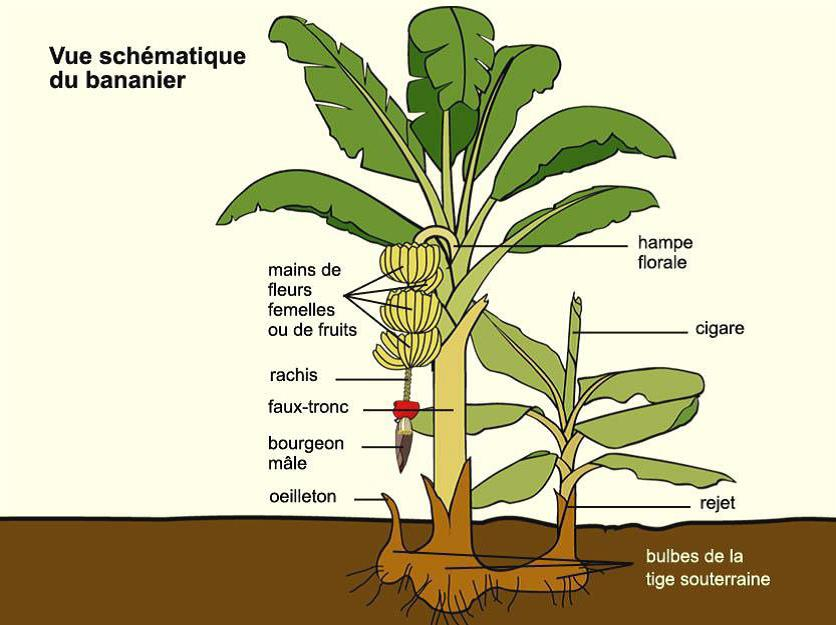
\includegraphics[scale=0.5]{banane}
	\captionof{figure}{Vue schématique d’un bananier à sa fructification et de ses rejets d’après  \cite{champion1967notes}}
\end{figure}

\section{Ravageurs}
\noindent{Parmi les principaux ravageurs des bananiers, se trouvent les nématodes pouvant provoquer des dégâts significatifs selon le milieu et le lieu géographique (\cite{gowen1990nematode}). Le nématode \textit{Radopholus similis} est le plus répandu (\cite{sarh1996nematode}). \textit{Pratylenchus coffeae} et \textit{Pratylenchus goodeyi} provoquent autant de dégâts mais sont moins répandus et relativement peu fréquents sur les bananiers (\cite{bridge1997nematode}). Tous ces nématodes ont un impact sur la production de bananes dans les tropiques alors que le nématode à spirale, Helicotylenchus multicinctus, provoque plus de dégâts dans la zone subtropicale (\cite{mcsorley1986nematological}). Le charançon, \textit{C. sordidus}, est l’insecte qui est le plus répandu et a le plus grand impact sur les bananiers (\cite{gold2001biology}).
}
\subsection{Lutte contre les charançons}
\subsubsection{Lutte chimique}
\noindent{Les pesticides sont d'un grand secours. Leur utilisation a été forte entre 1950 et 1986, les pays en développement utilisant le quart de tous les pesticides consommés dans le monde. Toutefois, un emploi incorrect et excessif de ces produits peut contaminer aussi bien les denrées alimentaires que l'environnement et, dans certains cas, nuire à la santé des agriculteurs (\cite{fao1996insecte}).}

\noindent{Jusqu'aux années 90, la principale technique de lutte contre le charançon était chimique. On retrouvait l'utilisation des fongicides et autres. Aux Antilles Françaises, le chlordécone, pesticide organochloré, était le plus utilisé (\cite{vilardebo1974chlordecone}), avant son interdiciton en 1993 du fait de sa toxicité et de sa forte persistence.}

\subsubsection{Piégeage de masse}
\noindent{Le piégeage de masse consistant à placer des pièges à phéromones dans les bordures des parcelles parcelles afin de limiter la contamination des parcelles avoisinantes (\cite{rhino2010effect}) est aussi un moyen de lutte contre les ravageurs mais, le rayon d'action des pièges et les facteurs influençant l'efficacité du piégeage sont encore méconnus et nécessitent des études approfondies afin d'optimiser la disposition spatiale des pièges à l'échelle de la parcelle, voire du réseau de parcelles.}

\noindent{Face aux pollutions graves liées à la lutte chimique , la résistance des ravageurs à ces méthodes de luttes et la non maîtrise des facteurs influençant l'efficacité du piégeage il urge de trouver de trouver une méthode alternative naturelles de lutte contre les ravageurs.}

\subsubsection{Système de lutte par un prédateur}
\noindent{Les agroécosystèmes diversifiés fournissent de nombreux services à l’homme dont la régulation biologique. L’association des cultures est une pratique agricole qui favorise la diversité des plantes dans les agroécosystèmes, fournit des ressources alimentaires alternatives et structure les communautés des arthropodes. Elle favorise les prédateurs généralistes pour la régulation biologique des ravageurs (\cite{dassou2014effet}).
}

\noindent{La régulation des charançons par contrôle biologique a fait l’objet de plusieurs études (\cite{gold2000biology}, \cite{collard2018spatial}, \cite{dassou2014effet}), bien que rare sont celles qui portent sur le Bénin}

\noindent{Les études sont menées, sur les ennemis naturels du charançon \textit{C. sordidus} afin d’identifier leur efficacité. Les ennemis naturels de \textit{C. sordidus} sont les arthropodes, les nématodes entomopathogènes, ainsi que des champignons entomopathogènes (\cite{gold2000biology}). Plusieurs coléoptères prédateurs qui se nourrissent des  larves du charançon ont été identifiés dans son aire d’origine, l’Asie du Sud – Est. Toutefois des difficultés subsistent pour introduire ses ennemis naturels dans d’autres zones de production (\cite{gold2000biology}). Par contre, l’utilisation des fourmis \textit{myrmicines Tetramorium guinense} et \textit{Pheidole megacephala} dans la lutte contre le charançon \textit{C. sordidus} dans les plantations de Cuba ont connu une efficacité (\cite{gold2000biology}). Les adultes et les larves du charançon dans les champs sont attaqués par les nématodes \textit{entomopathogènes Steinerma et Heterorhabditis spp}., mais ne sont efficaces qu’en fortes densités du charançon.
	
Certaines espèces de fourmis sont connues pour être responsables d’une régulation des populations de \textit{C. sordidus} (\cite{abera2007composition, abera2008experimental}; \cite{gold2001biology}), des taux de prédation
pouvant aller jusqu’à 70\%, comme il a été constaté à Cuba (\cite{perfecto1998deployment}). Les fourmis du genre \textit{Pheidole} ainsi que l’espèce \textit{Ondotomachus troglodytes} sont capables d’extraire naturellement des œufs de charançons dans les bananiers. Il a été également observé à plusieurs reprises des fourmis \textit{Pheidole} s’attaquant à des charançons adultes et les ramenant à leur nid (observation personnelle lors de la collecte des données)

De même, le \textit{dermaptère E. caraibe}, prédateur généraliste des bananeraies de la Martinique, a été testé contre les charançons du bananier (\cite{collard2018spatial}). Il a été constaté que l’abondance et l’activité des \textit{dermaptères} semblaient dépendre fortement des types d’habitats : les résidus de bananiers apparaissant particulièrement plus favorables aux \textit{dermaptères} que le sol nu(\cite{collard2018spatial}).}

\noindent{Afin d’étudier le rôle de la biodiversité, il est important de déterminer quelles sont les cultures présentes dans un écosystème donné et les relations entre elles. Nous étudierons ici l'association de la culture de maïs dans les bananeraies de Toffo}

\section{Modélisation et agroécologie}
\noindent{Il existe différents types de modèles en écologie, chacun ayant des avantages et des inconvénients. Les modèles les plus classiques sont des modèles agrégés, basées sur des équations différentielles ordinaires (EDO) ou partielles (EDP). Ces équations relient l’état d’un système à un instant t à des instants antérieurs. L’état du système est défini par une ou plusieurs variables quantitatives, parmi lesquelles des variables agrégées qui représentent le comportement d’un groupe d’individus, comme la biomasse ou le nombre d’individus (\cite{holt1977predation}; \cite{watson2015exploring}). Les équations de Lotka-Volterra ont été mobilisées pour étudier l’interaction du proie-prédateur dans le cadre du contrôle biologique des ravageurs. Le modèle macro est définie par les équations suivantes :
}

\begin{equation}
	\left\lbrace\begin{aligned}
		\dfrac{dx(t)}{dt}	& = x^{'}(t) = \dot{x} = ax(t)-bx(t)y(t)		\\
		\dfrac{dy(t)}{dt}	& = y^{'}(t) = \dot{y} = -cx(t)-bx(t)y(t)
	\end{aligned}\right.
\end{equation}
$$\systeme{\frac{dx(t)}{dt} = x^{'}(t) = \dot{x} = ax(t)-bx(t)y(t),,\frac{dy(t)}{dt} = y^{'}(t) = \dot{y} = -cx(t)-bx(t)y(t)}$$


\noindent{$x :$ nombre de proies\\
	$y : $ nombre de prédateurs\\
	$dx(t)/dt :$ variation du nombre de proies dans le temps\\
	$dy(t)/dt :$ variation du nombre de proies dans le temps\\
	$a :$ taux de natalité des proies\\
	$c :$ taux de mortalité des prédateurs\\
	$b :$ taux de mortalité des proies lié à la prédation\\
	$d :$ taux de natalité des prédateurs lié à la consommation de proies.\\
}

\noindent{Ces approches peuvent aussi représenter l’espace de manière explicite, où les déplacements des individus ou de leur biomasse sont assimilés à des processus de diffusion (\cite{okubo1980diffusion}; \cite{corbett1993role}; \cite{vinatier2013explaining}).
}

\noindent{De multiples arthropodes peuvent envahir une bananeraie grâce aux cultures associées. Un modèle spatialement explicite permettrait de prendre en compte l'effet des différents arthropodes rencontrés sur les bioagresseurs.\\
Les modèles individu- ou agent-centrés (IBM ou ABM) sont des approches de résolution de problème ascendantes (« bottom-up ») dans lesquels chaque entité du système est représentée par un individu se comportant de manière indépendante des autres (\cite{fachada2015towards}). Nécessitant une implémentation informatique, ce type de modèle est apparu après les travaux de \cite{schelling1969models}. Suite à l’augmentation de la puissance des ordinateurs (\cite{grimm2013individual}), le modèle s'est généralisé à partir de quatre courants de recherche différents : l’écologie, l’informatique et l’ingénierie, les sciences cognitives et les sciences sociales (\cite{tang2010agent})}

\noindent{Le développement d’un modèle de simulation de l’épidémiologie de \textit{C. sordidus}, combiné avec des modèles de croissance végétale a permis d’améliorer l’arrangement spatial des parcelles et les stratégies de piégeage, en lien avec les mouvements du ravageur et leur dépendance à la qualité de l’habitat travers le modèle COSMOS (\cite{vinatier2010dynamique}).\\
Le modèle développé est un modèle individu centré multi-agent. La création d'un système multi-agents consiste à reproduire un monde artificiel qui ressemble au monde observé - c'est-à-dire qu'il est composé de différents acteurs - à des fins expérimentales. Chaque agent est représenté comme une entité informatisée indépendante capable d'agir localement en réponse à des stimuli ou à la  communication avec d'autres agents.}

\section{Modèle spatialement explicit COSMOS}
\noindent{Le modèle COSMOS, vise à simuler l'épidémiologie spatiale de \textit{C. sordidus} à long terme en décrivant la dynamique de sa population et l'infestation des plantes hôtes qui en résulte. Le modèle considère tous les stades de l'insecte simultanément et suppose qu'il existe des variations individuelles de comportement en fonction de chaque stade de développement. Le modèle fonctionne selon l’hypothèse que la distribution des populations et des attaques de C. sordidus dans les champs de bananiers peut être modélisée selon des règles épidémiologiques identifiées au niveau individuel et calibrées à partir de la littérature. Le modèle COSMOS, comme le modèle SIMBA-NEM , centré sur les nematodes et le modèle SIMBA-CC sur les plantes de couvertures (\cite{tixier2008simba}; \cite{tixier2004simba}), vise à combler le fossé entre l'écologie comportementale individuelle et la dynamique des populations (\cite{deangelis1994individual}).  Il a été validé en comparant les sorties du modèle avec les données de terrain. Enfin, COSMOS a été utilisé pour tester comment les schémas de plantation et l'hétérogénéité spatiale des stades de la plante, résultant de la variabilité de l'apparition des drageons au cours des cycles de culture, pouvaient modifier le temps nécessaire à la colonisation de l'ensemble de la parcelle et le niveau des dégâts pendant trois cycles de culture, lorsque la population initiale de charançons était distribuée le long d'un côté de la plantation.}


%---------------------------------------------------------------------------------------

% Define some commands to keep the formatting separated from the content
\newcommand{\keyword}[1]{\textbf{#1}}
\newcommand{\tabhead}[1]{\textbf{#1}}
\newcommand{\code}[1]{\texttt{#1}}
\newcommand{\file}[1]{\texttt{\bfseries#1}}
\newcommand{\option}[1]{\texttt{\itshape#1}}

%---------------------------------------------------------------------------------------


% Chapter 2

\chapter{Matériels et méthode} % Main chapter title
\label{Chapter3} % For referencing the chapter elsewhere, use \ref{Chapter1}
%\minitoclt
\section{Zone d’étude}
\noindent{Pour mener notre étude, nous avons choisi la zone de production bananière de Toffo. Cette zone a été choisie, surtout, à cause de la diversité des champs de bananier. On y retrouve d'autres cultures associées telles que le maïs, la canne à sucre, le niébé, le papayer, l'oranger... }

\noindent{La commune de Toffo concernée par notre étude est située dans la zone septentrionale du département  de l’atlantique avec une superficie de 492 $km^2$ environ $15\%$ de la superficie du département, et $0,42\%$ de la superficie totale du Bénin. Elle est limitée au Nord par la commune de Zogbodomey dans le département du Zou, au Sud par la commune d’Allada, à l’Est par la commune de Zè (au Sud-Est) et à l’Ouest par le fleuve Couffo servant de frontière naturelle avec la commune de Lalo dans le département du Couffo. La commune de Toffo est subdivisée en 10 arrondissements, décomposés en 54 villages. Le chef-lieu de la commune est  l’arrondissement de Toffo-centre situé à environ  81km de Cotonou (\cite{adjovi2006localisation}).}
\begin{figure}
	\centering
	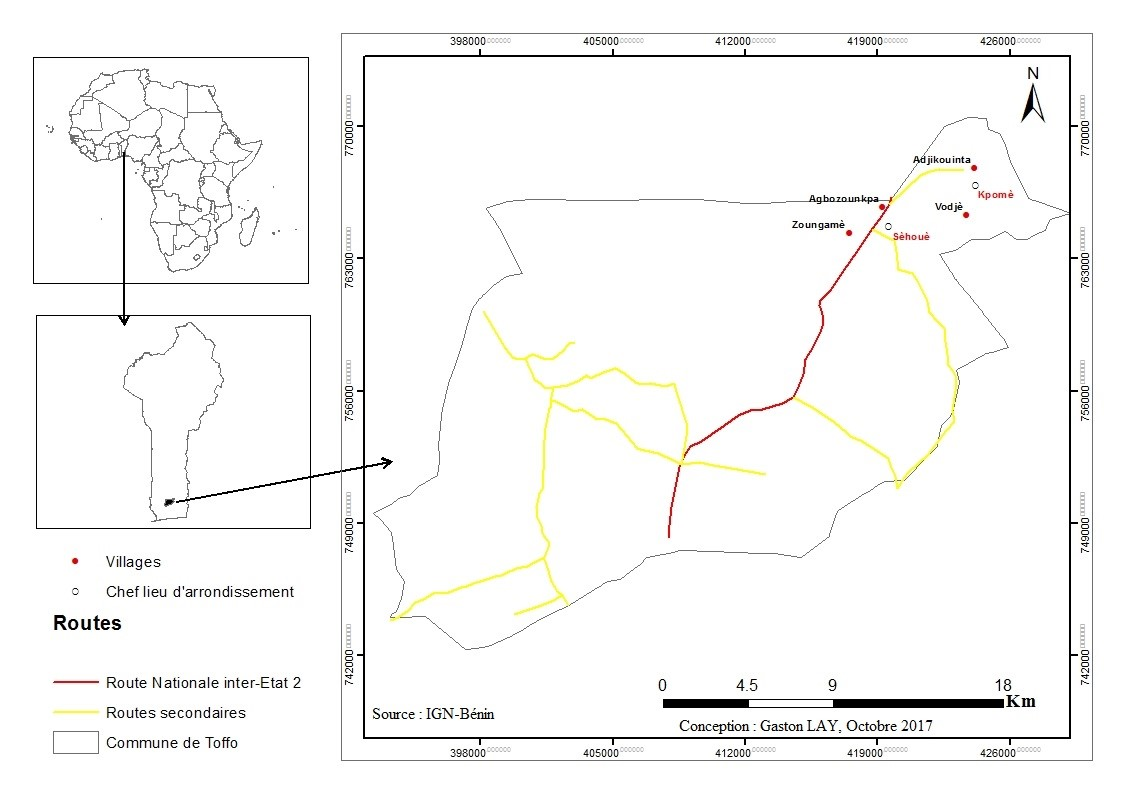
\includegraphics[scale=0.5]{carte}
	\captionof{figure}{Carte de la commune de Toffo}
\end{figure}
\section{Collecte des données}
\noindent{Nous utilisons dans ce travail comme données, les mesures de prédations journalières dans les champs de bananiers de Toffo allant de 15 août au 5 septembre 2021. Ces données sont obtenues par protocole de proie sentinelle (\cite{ricci2017cartes}). }
\subsection{Protocole de « proie sentinelle » }
\noindent{Le principe d’une proie sentinelle est d’exposer aux prédateurs des proies et de mesurer la proportion de proies consommées après un temps donné. Ici, nous utiliserions des charançons vivants que l’on entrave avec un petit fil de pêche, lui-même fixé au sol. La mesure consiste à noter la présence ou l’absence du charançon après 24h d’exposition. On dispose des petits morceaux de feuille de bananier pour offrir un abri au charançon, mais pas trop grand pour qu’ils restent exposés à certains moments (par exemple 4 morceaux de 4cm de côté).}
\begin{figure}
	\centering
	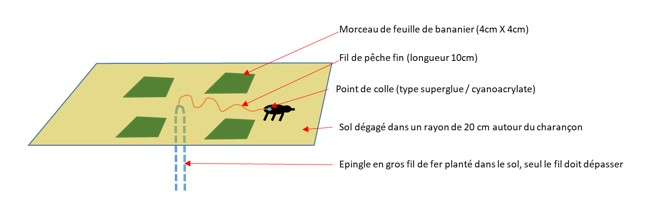
\includegraphics[]{proiesentinelle}
	\captionof{figure}{Protocole de proie sentinelle}
\end{figure}

\noindent{Une estimation du ratio de prédation peut être obtenue en confinant la proie et les prédateurs dans une cage placée au champ en conditions réelles. La limite de cette méthode est qu’elle ne donne pas d’indication sur la nature des prédateurs, elle ne donne qu’une estimation globale du ratio de prédation aux pieds des bananiers et des maïs, tous prédateurs confondus (\cite{mollot2012new}).}
\subsubsection{Méthodologie}
\noindent{Afin de simplifier l’approche, les cultures associées ont été restreintes à une culture la plus couramment rencontrée dans la zone étudiée (le maïs). Nous utilisons donc d’une approche par proies sentinelles afin d’estimer la prédation des adultes. La proie sentinelle a été déposée toujours à la même distance du bananier et de la plante associée. Nous procédons ensuite à la campagne de mesure de la prédation sur un réseau de parcelles avec à chaque fois la quantification de la prédation en zone proche des bananiers ou proche de la culture associée, en faisant à chaque fois des mesures appariées (bananier \& culture associée).\\
Vingt parcelles diversifiées (on observe la présence du maïs avec d'autres cultures telles que la canne à sucre, le niébé, le papayé, l'oranger...) ont été explorées avec cinq couples de charançons par parcelle. Les parcelles ont une longueur d’au moins 25m de côté afin de réaliser les mesures plus au centre pour limiter les effets de bord. La mesure dure 24 heures.
}
\begin{figure}
	\centering
	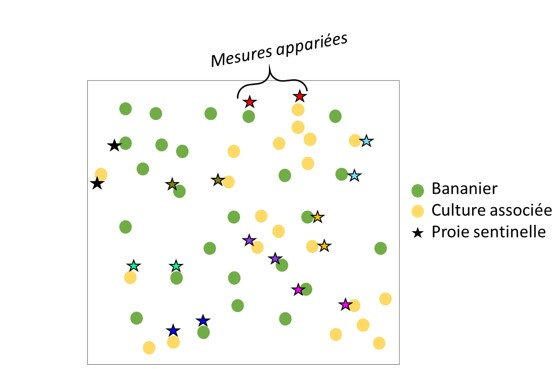
\includegraphics[]{placement}
	\captionof{figure}{Disposition de proie dans les champs}
\end{figure}
\begin{figure}
	\centering
	\includegraphics[height=15cm]{terrain}
	\captionof{figure}{ a)Photo de charançons attachés avant exposition dans le champ, b) Le charançon au début de son exposition dans le champ, c) Le champ d’exposition et d) Charançon consommé à 70\% après 24h  d’exposition dans le champ.}
\end{figure}

\section{Analyse statistique des taux de prédation de charançons dans un champ de bananier-maïs}
\noindent{Une base de données a été analysée  dans le but de s’informer sur le ratio de prédation entre les cultures de bananiers et maïs. Toute l’analyse statistique a été réalisée avec le logiciel \cite{rcitation}. Ce choix repose sur l’accessibilité du logiciel, ses mises à jours et l’accès à de nombreux packages  (utilisation notamment des packages lme4 \cite{lme4}, sjPlot \cite{sjplot} et emmeans \cite{emmeans}).}

\noindent{L’hypothèse d’indépendance des données n’étant pas vérifiée , le modèle choisit est donc le modèle linéaire mixte généralisé (GLMM ) (\cite{zuur2009mixed}). Ce modèle est une extension du modèle linéaire généralisé permettant la corrélation entre les observations et des données imbriquées.}

\noindent{Le seul effet aléatoire considéré est le champ. Nous ne cherchons pas à comprendre la prédation des charançons à l’échelle du paysage mais leur prédation dans de champ à petite échelle. Pour ce faire, nous utiliserons les groupes déterminés dans les champs, ce qui nous permettra de regrouper des états initiaux similaires. Le jeu de données tiré du protocole présente des données sur la régulation naturelle du charançon du bananier dans 20 parcelles de bananiers et maïs à Toffo. La prédation (Pred) a été mesurée pour cinq (5) couples de charançons sur chacune des 20 parcelles (champ) pour un total de 200 observations. La variable density mesure la densité de chaque parcelle en bananiers par rapport à la densité moyenne, tandis que la complexité de l'agro-écosystème est mesurée à l’échelle de la parcelle.
	
Les autres cultures souvent rencontrées sur les parcelles étant des tecks, papayés, orangers et palmeraies. La complexité agro-écologie a été calculée comme une variable de niveau qui exprime le nombre de cultures retrouvées dans la parcelle. La complexité est initialisée à 1 pour toutes les parcelles à cause de la présence du maïs. La complexité est donc la somme des variables binaires (absence ou présence des autres cultures sur une parcelle donnée)
	
Puisque la prédation représente la mort ou pas des charançons dans une parcelle, nous pouvons modéliser cette réponse par une régression binomiale, avec un effet fixe de la densité et un effet aléatoire du champ sur les deux coefficients. Le modèle suivant est appliquée sur nos données}

$logit(P_{ij})=\alpha + \beta_0*cult_{ij} + \beta_1*density_{ij}*complexite_i + \beta_2*champ_i$

\noindent{La notation logit correspondant au lien logistique (zuur2009mixed), $P_{ij}$ est la probabilité que le charançon j du champ i et de complexité i soit mort par prédation, $cult_i$ nous indique la plante hôte du charançon  (s'il s'agit d'un bananier ou du maïs), $complexité_i$ identifie la complexité agro-écologique et $champ_i$ identifie la parcelle. $density_{ij}$ est la densité de bananiers dans les champs.
	
La significativité des variables du modèle est testé en les supprimant à tour de rôle afin de comparer deux à deux le critère d'information d'Akaike (AIC) du modèle initial avec celui des sous-modèles. L’AIC mesure la qualité d’ajustement et la complexité du modèle (\cite{zuur2009mixed}) et est défini par l’équation suivante : $$AIC= -2\ln(L(\theta))+2K$$
avec $k$ le nombre de paramètres et $\theta$, la vraisemblance maximisée du modèle.\\
Pour chaque test réalisé, le seuil de significativité est de 0,05.	
}

\subsection{Résultats et discussion}
\begin{verbatim}
Single term deletions

Model:
pred ~ cult + density * complexity + (1 + density | champ)
				   npar    AIC    LRT  Pr(Chi)   
<none>                  274.01                   
cult                  1 279.88 7.8719 0.005021 **
density:complexity    2 270.03 0.0214 0.989347   
---
Signif. codes:  0 ‘***’ 0.001 ‘**’ 0.01 ‘*’ 0.05 ‘.’ 0.1 ‘ ’ 1
\end{verbatim}
\noindent{L'AIC pour le modèle dans lequel aucun terme n'est supprimé est de 274.01. En supprimant la variable nominale cult (culture) de ce modèle, l'écart augmente à 279.88, soit une variation de 5.87. La variation de déviance pour le GLM binomial est distribuée par un chi carré avec 1 degré de liberté et a une p-value inférieure à 0,01, ce qui signifie que le terme est  significatif. En supprimant le terme d'interaction seul, on observe une réduction de 3.98 de l'AIC et qui n'est pas significatif. \\
	Pour avoir une idée de ce que fait le modèle, nous avons voulu visualiser les valeurs prédites.}
\begin{figure}
	\centering
	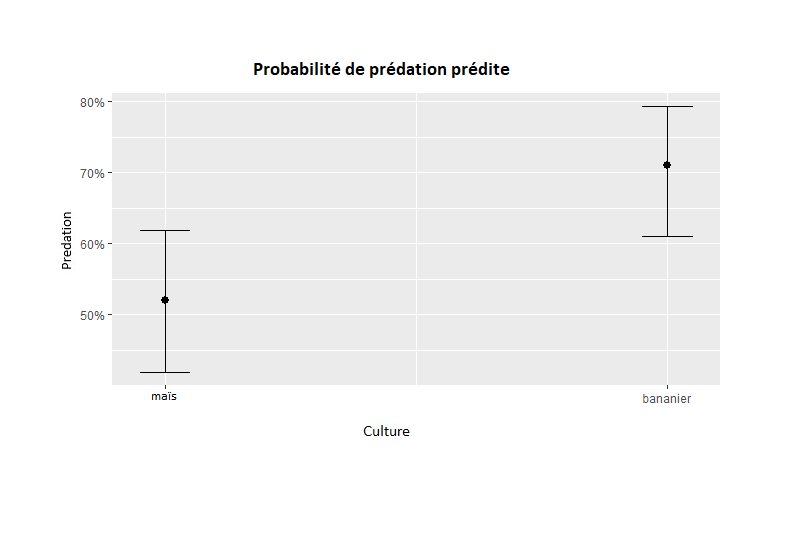
\includegraphics[height=12cm]{ratio}
	\captionof{figure}{\label{rat}Taux de prédation des charançons aux pieds des bananiers et des maïs dans les champs.}
\end{figure}

\noindent{la figure \ref{rat} nous informe sur le taux de prédation des ravageurs aux pieds des bananiers et des maïs. La moyenne aux pieds des maïs est d'environ 52\% et 71\% pour le bananier. L’exposition de proies sentinelles est une technique relativement biaisée par rapport à la prédation naturelle de ravageurs (proies mortes, messages d’odeurs agrégation ou surexposition plus ou moins volontaire des proies) \cite{ricci2017cartes}. Ceci nous amène à considérer un rapport de prédation entre le taux de prédation au pieds des bananiers et des maïs et ceci sur une durée de vie des charançons. Nous considérons donc un ratio de 52/71}

\begin{figure}
	\centering
	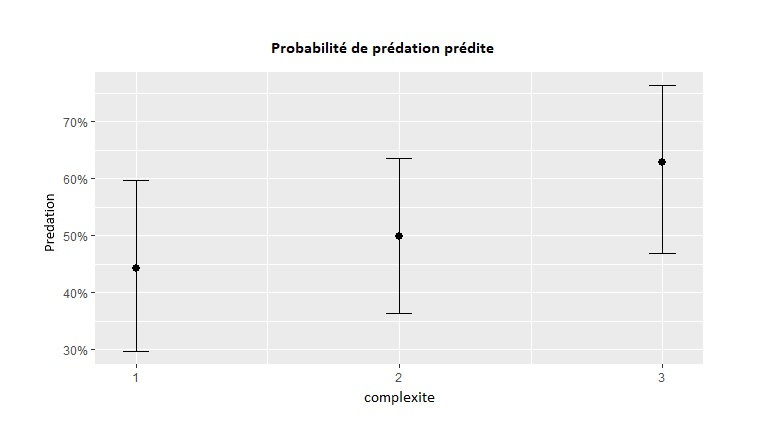
\includegraphics[height=10cm]{complexite}
	\captionof{figure}{\label{complec}Taux de prédation prédit par GLMM en fonction de la complexité  des champs.}
\end{figure}

\noindent{De ce graphique, on retient que dans les champs de bananiers et maïs uniquement (complexité = 1), il y a un taux moyen d’environ 0.45 de prédation pour un charançon donné (ce taux peut varier entre 0.3 et 0.6). Le taux moyen augmente au fur et à mesure que la diversité des parcelles devienne plus complexe. Tout ceci conforte l’hypothèse d’une régulation de charançons importante dans les champs avec les cultures associées (diversité agro-écologique complexe). \cite{ostman2001landscape} et de \cite{chaplin2011meta} font ressortir que dans la plupart des situations, les paysages plus complexes, comportant davantage d’habitats semi-naturels, sont associés à une plus grande abondance et à une plus grande diversité d’ennemis naturels, ce qui augmente donc la probabilité de prédation des ravageurs.
}
\begin{figure}
	\centering
	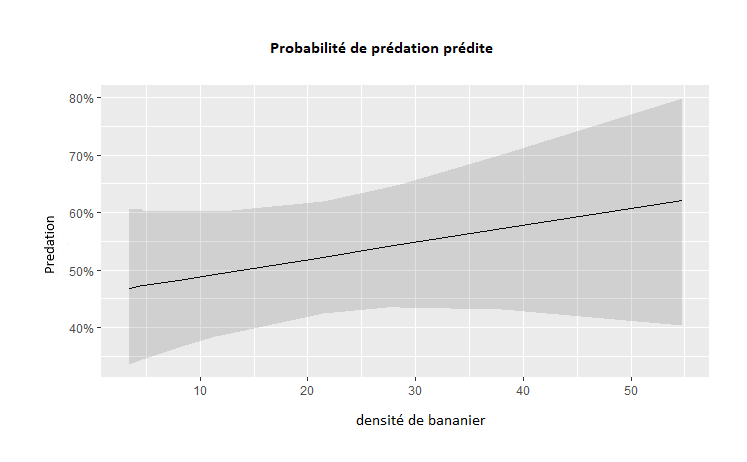
\includegraphics[height=10cm]{densite}
	\captionof{figure}{\label{dens}Taux de prédation prédite par GLMM en fonction de la densité bananiers dans les champs.}
\end{figure}
\noindent{La figure \ref{dens} nous montre le taux de prédation des ravageurs en fonction de la densité de bananiers dans les champs. On constate une tendance de moyenne linéaire qui croit avec la densité. En effet, la lutte par les ennemis n'est efficace qu'en présence d'une forte densité des ravageurs (\cite{gold2000biology}). On fait donc l'hypothèse que plus le champ est dense, plus on est susceptible d'avoir une forte densité de ravageurs aussi. Optimal foraging theory suppose que le prédateur cherche à obtenir le plus de ressources tout en minimisant le temps passé à chercher sa proie (\cite{davies2012introduction}). L’évolution des prédateurs vers le spécialisme ou le généralisme peut donc dépendre de la quantité de proies disponible. L’optimal foraging prédit que lorsque la ressource optimale est abondante, les prédateurs ont tendance à se spécialiser sur cette ressource, car ils perdent peu d’énergie à chercher leur proie optimale (\cite{davies2012introduction}).}

\subsection{Conclusion }
\noindent{Dans le but de lutter contre les ravageurs, la complexité de l’agrosystème s’est avérée comme un bon moyen de régulation naturelle. De plus, ces qualités en tant qu’un service de régulation biologique ont déjà été appréciées dans d’autres études. Nous nous basons donc, sur le ratio de prédation pour proposer un modèle mécaniste simulant la prédation des \textit{C. sordidus}. pour différentes configurations d'association de culture de bananier avec le maïs.}

\section{Modèle mécaniste COSMOSPARK}
\noindent{Le modèle vise à simuler les pratiques agricoles et son environnement animal et végétal dans le but de prédire l’évolution des populations de bioagresseurs et d’éviter leur installation. Nous nous sommes intéressés ici aux bananeraies intercalé avec le maïs et à leur ravageur principal, le charançon \textit{Cosmopolites sordidus}. Le modèle Cosmospark basé sur les individus a été implémenté dans NetLogo (\cite{tisue2004netlogo}), et sa description est détaillée en utilisant le protocole ODD (\cite{grimm2010odd} ; \cite{grimm2013individual})}
\subsection{Description et paramétrage du modèle}
\noindent{Le modèle est basé sur des données de présence-absence de charançons dans un ensemble d'habitats. Ces données instantanées sont collectées sur une seule génération (les adultes) et sont supposées représenter le quasi-équilibre de la dynamique des métapopulations. L'objectif de la modélisation est d'ajuster la fonction d'incidence aux données instantanées observées, afin d'obtenir des estimateurs des paramètres du processus spécifique aux\textit{C. sordidus}. Une fois ces paramètres connus, le modèle peut être utilisé pour prédire les probabilités de prédation spécifiques à l'habitat pour une configuration particulière de l'habitat. Ainsi, les taux de prédation peuvent-être prédits pour chaque type d’habitat. Cette prédation est supposée se produire au hasard pour chaque habitat.
	
\begin{table}
	\small
	\caption{\label{parametre}Paramètres du modèle. Ces paramètres proviennent du modèle de base. Nous ajoutons ici, le taux de prédation au pied de bananier. }
	\begin{tabular}{L{5cm} @{} C{1.5cm} @{} C{1.5cm} @{} C{5cm} @{} L{3cm} }
		\hline Description & Code & Valeur &Intervalle utilisé pour l’analyse de la sensitivité & références\\
		\hline \textbf{Adult} & & & &\\
		Sex-ratio (male:female) & -- & 1:1 & -- & \cite{gold2001biology}\\
		Sexual maturity for females after
		emergence (days) & SM & 34.5 & 33-36 & \cite{cuille1950recherches}\\
		Probability of egg-laying on 
		maiden sucker compared to flowered plants & OMPS & 0.11 & 0.08-0.13 & \cite{abera1997oviposition}\\
		Probability of egg-laying on
		preflowered plants compared to
		flowered plants & OPPF & 0.41 & 0.39-0.46 & \cite{abera1997oviposition}\\
		Number of adults per week
		necessary for density-dependent effect
		on fecundity & DE & 20 & 10-33 & \cite{abera1997oviposition}\\
		Number of eggs per week per female
		without density-dependent effect & FH & 2.7 & 1.7-3.2 & \cite{koppenhofer1993observations}\\
		Number of eggs per week per female
		with density-dependent effect & FL & 0.8 & 0.6-1.1 & \cite{abera1997oviposition}\\
		Maximum lifespan of adult (days) & ML & 748 & 542-748 & \cite{froggatt1926banana}\\
		Proportion of individuals moving 2 m
		per time step (\%) & DC1 & 1.4 & 1.5-6.6 & \cite{delatre1980insect}\\
		Proportion of individuals moving 4 m
		per time step (\%) & DC2 & 0.3 & 0.0-3.0 & \cite{delatre1980insect}\\ 
		& & & & \\
		\textbf{Banana plant} & & & & \\
		Banana maize predation & BMP & 0.03 & 0.02-0.2 & --\\
		Interval planting–maiden sucker
		(degree-days) & -- & 800 & -- & \cite{abera1997oviposition}\\
		Interval planting–preflowering
		(degree-days) & -- & 1600 & -- & \cite{abera1997oviposition}\\
		Interval planting–post-flowering
		(degree-days) & -- & 2350 & -- & \cite{tixier2004simba}\\ 
		\hline 
	\end{tabular}
\end{table}
}


\subsection{Caractéristiques générales du modèle COSMOSPARK}
\noindent{Le modèle COSMOSPARK est un IBM stochastique qui fonctionne sur un pas de temps quotidien. C’est une extension du modèle COSMOS (\cite{vinatier2009cosmos}) simulant le mouvement local et la ponte des femelles dans le champ, l'infestation des larves dans les bananiers, et les principales caractéristiques du développement de l'insecte et de la plante hôte. COSMOSPAK intègre à cet effet la prédation des charançons adultes en ajoutant une culture favorable à la prédation (le maïs). Selon le modèle, les individus \textit{C. sordidus} se dispersent dans un champ représenté par une grille avec un bananier par cellule (la surface de la grille varie entre 144 et 441 m2). Les plantes de bananiers passent par trois étapes distinctes jusqu'à la récolte : le drageonnage, la préfloraison et la post-floraison. Juste avant la floraison, on sélectionne un nouveau drageon de la plante mère qui pousse simultanément dans la même cellule. Le délai entre deux récoltes consécutives, correspondant à un cycle de culture, est d'environ 200 jours (voir \cite{tixier2004simba} pour des détails sur les cycles de culture du bananier). Les femelles de \textit{C. sordidus} pondent des œufs sur les bananiers, et les larves issues de ces œufs percent le cornet des plantes. La durée des stades des juvéniles et les stades phrénologiques des bananiers dépendent de la température. Les plantes de maïs sont considérées comme statique dans le modèle faisant apparaitre une mortalité par prédation. Les prédateurs ont été caractérisés par un "effet prédation" distribué sur les cellules de plantes en fonction de la proximité de maïs. La figure \ref{uml} présente le modèle et ses caractéristiques. }
\begin{figure}
	\centering
	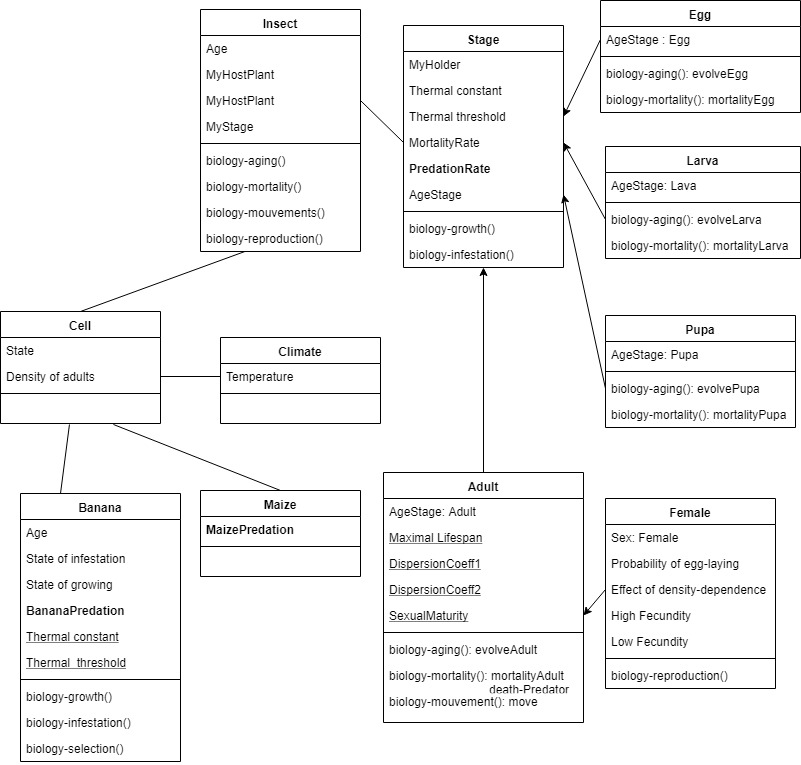
\includegraphics[height=15cm]{UML_COSMOSPARK}
	\captionof{figure}{\label{uml} Diagramme de classes du modèle COSMOSPARK.}
\end{figure}

\subsection{Protocole ODD}
\subsubsection{Présentation générale}
\paragraph{Objectif}$ $ \\

\noindent{Le but de notre modèle est de simuler la prédation de \textit{C. sordidus} par les arthropodes prédateurs en décrivant comment des patterns d’organisation spatiale (bananiers \& culture associées) modifient la dynamique des populations de charançon sur une parcelle donnée.}
\paragraph{Entités, variables d'état et échelles}$ $ \\

\noindent{Le modèle COSMOSPARK comporte 3 entités, les charançons, les bananiers, les maïs. Les charançons sont décrits par 3 variables d’état : l’emplacement –x, y – leur stade de vie et leur sexe. Les bananiers sont décrits par leur emplacement (cellule de grille) et une liste numérique contenant le taux de mortalité journalier sur chaque bananier en fonction de sa configuration. Les maïs aussi sont décrits par leur emplacement (cellule de grille) et une liste numérique contenant le taux de mortalité journalier fixe sur chaque maïs. Les unités spatiales sont caractérisées par leur emplacement (cellule de grille) et leur type d'habitat. Les deux types d’habitats sont les habitats de culture contenant bananiers et maïs (habitat favorable aux prédateurs).  L’habitat proche de culture de maïs est considéré comme favorable à la régulation des charançons et donc a d’effet sur les charançons.Les parcelles de champ de bananiers- maïs dans le modèle sont de 25 m x 25 m et ont un grain de 2 x 2 m. La superficie de la parcelle a été choisie pour faciliter la prise en compte de divers modèles spatiaux de cultures et d'un nombre et d'une densité raisonnables de plants de bananes (1736 plants de bananes /ha ; Vinatier et al, 2009). Une parcelle est alors une grille carrée de 50 x 48 cellules traitée comme un tore. Tous les bananiers et les mais sont placés sur des cellules côte-à-côte les uns des autres pour limiter l’effet du sol nu.
Les charançons ont une durée de vie en moyenne de deux ans. Le modèle fonctionne sur un pas de temps journalier pendant deux ans donc, 748 jours.}
\begin{figure}
	\centering
	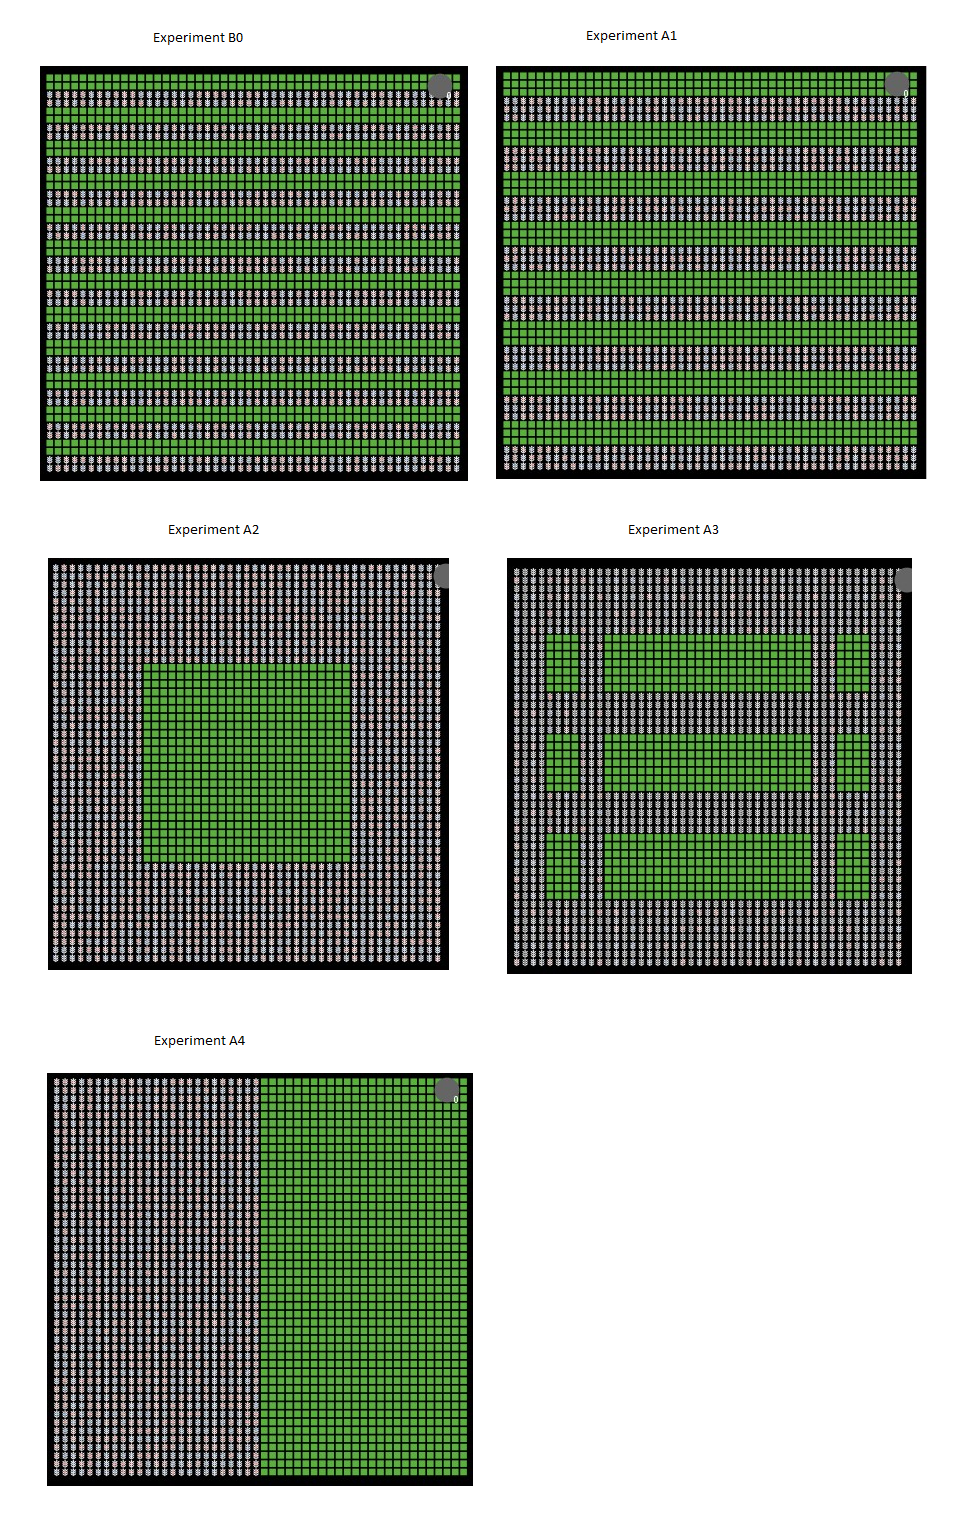
\includegraphics[width=12cm]{Patterns}
	\captionof{figure}{\label{patterns} Les patterns du modèle. Les bananiers sont en blanc et les maïs en vert. Les charançons ont été disposés aux pieds de bananiers.}
\end{figure}

\paragraph{Vue d'ensemble du processus et ordonnancement}$ $ \\

\noindent{Les processus de simulation du modèle sont décrits dans l'organigramme (Fig. \ref{flowchaart}). A chaque pas de temps, deux sous-modèles sont exécutés dans l'ordre suivant : La prédation et l'observation des bananiers. La prédation est exécutée pour tous les ravageurs dans un ordre aléatoire et défini le fait qu'ils soient tués ou pas en fonction de la configuration du champ. Le sous-modèle Observation des bananiers est ensuite exécuté pour tous les bananiers dans un ordre aléatoire et enregistre le nombre de ravageurs présents dans la parcelle.}
\begin{figure}
	\centering
	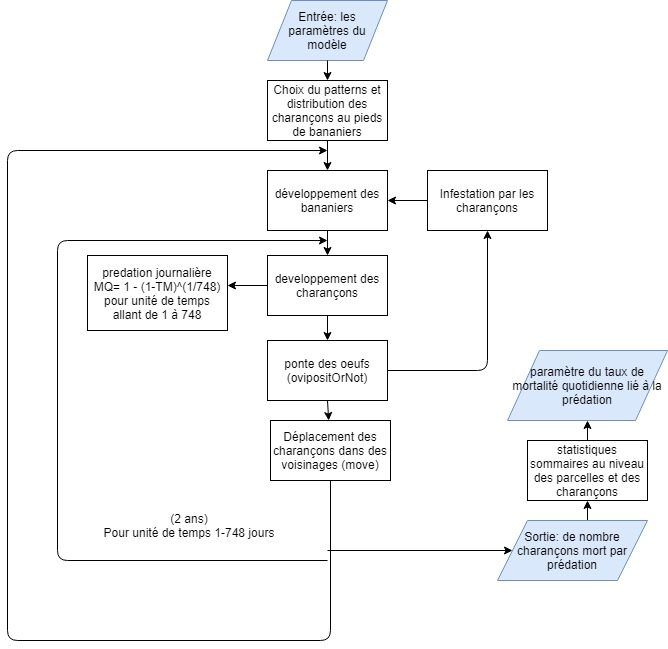
\includegraphics[width=12cm]{flowchart}
	\captionof{figure}{\label{flowchaart} Organigramme du modèle de simulation examinant la relation entre l’organisation des parcelles et le taux de prédation.}
\end{figure}
\subsubsection{Concepts de conception}
\noindent{\textit{Basic principles :} Le modèle est une extension du modèle COSMOS qui simule l'épidémiologie spatiale de \textit{C. sordidus} à long terme en décrivant la dynamique de sa population et l'infestation des plantes hôtes qui en résulte. L’ajout des maïs au modèle constitue un habitat favorable aux prédateurs généralistes dont l’effet a été modélisé par la fixation des taux, sur des patches, qui varient en fonction du type d’habitat.

\textit{Emergence :} La dynamique des mouvements des charançons et la pression de prédation qui en résulte sur l'ensemble des bananiers émergent du comportement de recherche de nourriture des individus. L'interaction entre les mouvements, l'effet dilution et l'organisation spatiale n'est pas simple.

\textit{Adaptation :} agents purement réactifs

\textit{Objectives :} agents purement réactifs

\textit{Learning :} agents purement réactifs

\textit{Prediction :} agents purement réactifs

\textit{Sensing :} Les bananiers sont sensible au climat. Les charançons ne peuvent percevoir que l'habitat où ils se trouvent au début de l'étape de temps et les habitats qu'ils traversent au cours de leurs déplacements aléatoires.

\textit{Stochasticity :} Dans le modèle, la construction des parcelles (simulation des parcelles), les mouvements individuels et les décisions de prédation sont stochastiques. Les mouvements sont classiquement modélisés par une chaîne de Markov de premier ordre. Par conséquent, la stochasticité a également été choisie pour les décisions des ravageurs de bouger.

\textit{Observation :} Pour une simulation (748 jours), les listes numériques des ravageurs sont importées de Netlogo vers R (\cite{rcitation}) via le package RNetlogo (\cite{thiele2014r}; \cite{thiele2012rnetlogo}). Les statistiques sommaires du nombre de ravageurs mort par prédation tenant compte de l’organisation spatiale ont été calculées via R (voir la définition détaillée des paramètres dans le tableau \ref{parametre}). Nous observons donc, la moyenne des infestations et la proportion de plantes sévèrement infectées en fonction des patterns.

\textit{Collectives :} Il n’y a pas de collectif mais, il y a une densité des charançons qui influe sur leur capacité à se reproduire.
}
\subsubsection{Détails}
\noindent{\textit{Initialisation :} Le modèle est initialisé en assignant des types d'habitats aux cellules (c'est-à-dire des simulations de parcelles), en spécifiant les paramètres prédation et en distribuant les ravageurs aux pieds des bananiers dans une parcelle.
	
\textit{Input data :} Il n’y a pas de données externes dans notre modèle mis à part les paramètres du modèle.
}

\paragraph{Sous-modèles} $ $ \\

 \noindent{ \textit{Move :} Le déplacement des  charançons est influencé par l’habitat dans lequel il se trouve. Les animaux utilisent une grande variété d'indices chimiques, visuels et acoustiques pour évaluer l'aptitude de l'habitat à fournir de la nourriture (\cite{searle2005should}), la ponte (\cite{rabasa2005egg}) ou la protection contre les prédateurs (\cite{hufker1999az}). La perception d’habitat par un individu est définie par le noyau de dispersion qui prend compte des contraintes de déplacement d’un habitat à un autre en fonction de la distance par rapport à l’emplacement actuel. Bien qu’ils soient considérés comme statique dans le temps et dans l’espace (\cite{chapman2007modelling} ; \cite{coombs2007field}), les noyaux de dispersion peuvent différer en fonction du temps (\cite{phillips2008reid}), de facteurs intrinsèques tels que le sexe, l'âge, le statut social ou les réserves énergétiques, et des conditions environnementales telles que le climat, la saison, la qualité de l'habitat, la compétition, la prédation et le parasitisme (\cite{bianchi2009foraging}; \cite{walters2006modelling}). En se servant des récentes avancées en matière de radiopistage des individus (\cite{schick2008understanding}), et en considérant le mouvement individuel des charançons comme une marche aléatoire dans laquelle les lieux d'arrivée et de départ des individus dépendent des caractéristiques de l'habitat et de leur distance par rapport à l'emplacement actuel de l'individu, (\cite{vinatier2010radiotelemetry}) ont défini la probabilité de déplacement d'une cellule a à une cellule b de la grille dans une unité temporelle par une chaîne de Markov de premier ordre définie par :
 $$Pr(a \rightarrow b)=\frac{\alpha_{h(b)}f_{\beta h}(d_{ab})}{\sum_{k=1}^{m}\alpha_h(k)f_{\beta h}()d_{ak}}$$

Où $\alpha_{(h(k))}$est la préférence relative pour l'habitat $h$ de la cellule $k$, $d_{ak}$ la distance entre les cellules $a$ et $k$ et $f(d_{ak})$ le noyau de dispersion dépendant de la distance définie par $exp^{((-\beta a.d_{ab}))}$ La décision individuelle de se déplacer a été basée sur une probabilité multinomiale entre toutes les probabilités calculées sur la grille. Pour l'efficacité du calcul, les cellules avec des probabilités proches de zéro n'ont pas été considérées dans la probabilité multinomiale.

\textit{Death-predator :} La mortalité due à la prédation est journalière et suit une distribution binomiale avec une probabilité dépendant de la configuration spatiale et du type d’habitat sur lequel se retrouve le charançon. Dans un champ de bananier avec maïs intercalé, le taux de prédation est censé suivre une distribution de poisson (\cite{hilker2006parameterizing}). Si le charançon se trouve sur un habitat bananier avec un l’habitat maïs situé à une distance de prédation (d) donnée, le charançon a une probabilité : $$p=1-(1-MQ)^{(\frac{1}{ML})} $$ d'être bouffé \cite{bousquet2001multiagent}.

Avec $MQ$ : la mortalité quotidienne et $ML$ : la durée de vie d’un charançon }
\subsection{Procédure de simulation}
\subsubsection{Validation du modèle}
\noindent{La simulation a été réalisée dans une zone de 52*52 cellules (dimension de cellules 2,4 *2,4). Chaque bananier appartenait à une cellule ainsi que chaque maïs. Le modèle a été rendu simple en ne laissant aucune cellule vide donc toutes cellules contenaient chacune un bananier ou maïs. Les simulations ont été effectuées sur 748 jours, correspondant à la durée de vie d’un charançon. Pour l’estimation du taux quotidien de mortalité, nous avons, dans un premier temps établi une relation pour calculer le ratio de régulation de la population de charançons aux pieds des bananiers et des maïs en utilisant les données obtenues par proie sentinelle dans les champs de bananeraies de Toffo. Le ratio de régulation de \textit{C. sordidus} était 52/71 dans un champ de bananiers avec maïs intercalé. Le taux de mortalité quotidien a été ensuite varié entre 0 et 1 sur les différents patterns (fig. \ref{patterns}). En analysant la figure, on constate qu’à partir de 0.2, on obtient  presque une croissance de charançons qui est quasi-nulle pour les cinq patterns.}
\begin{figure}
	\centering
	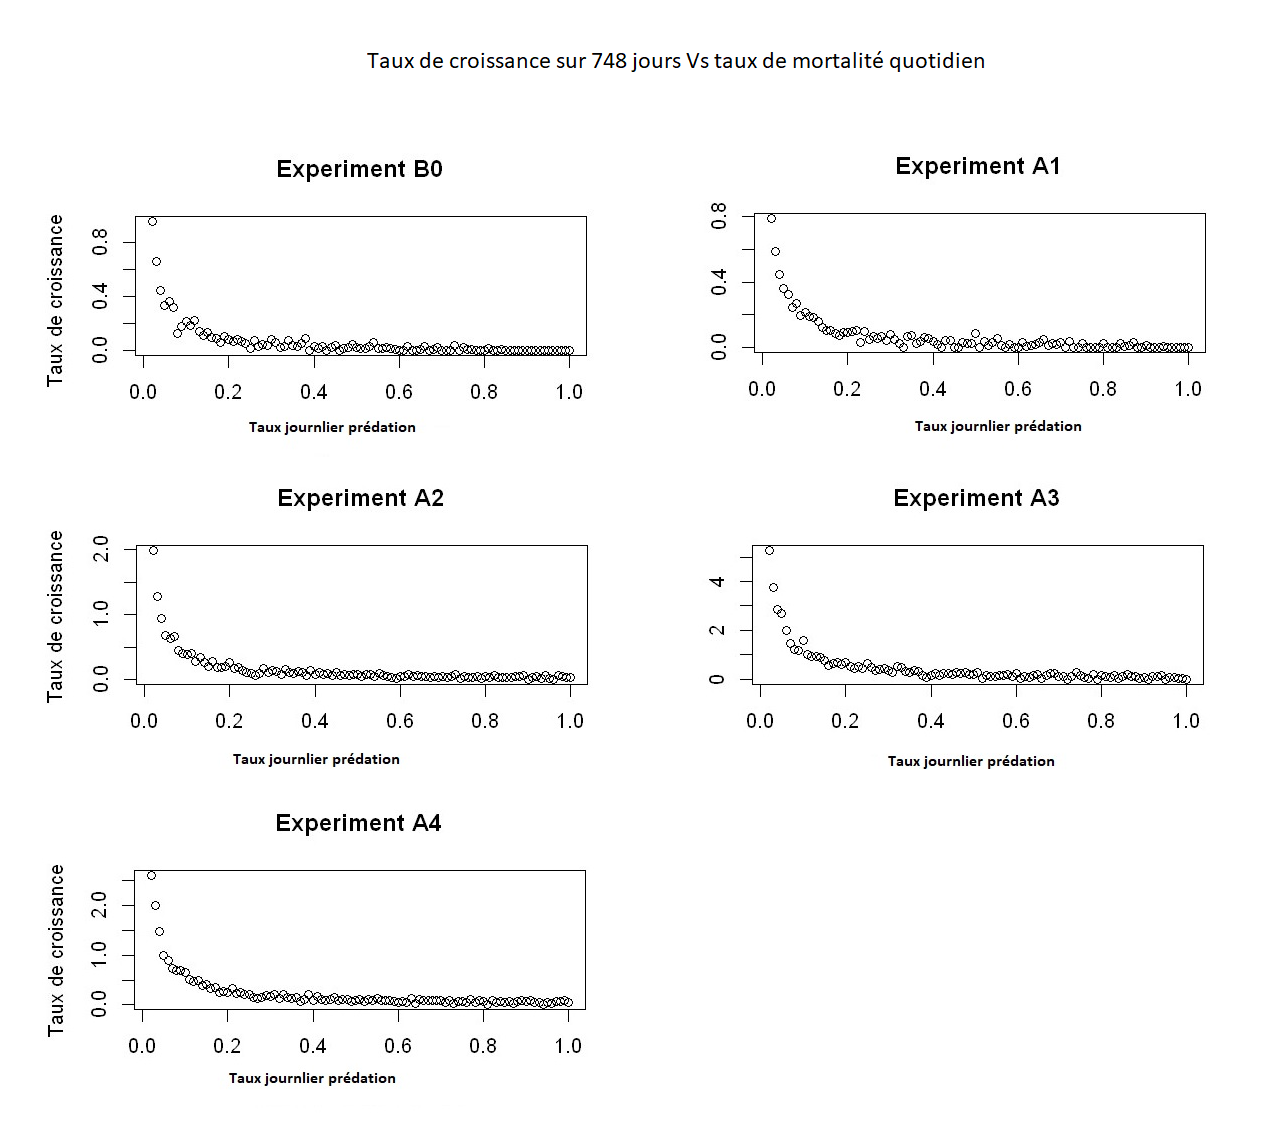
\includegraphics[width=17cm]{rate}
	\captionof{figure}{\label{taux} Recherche d'une approximation du taux de mortalité quotidien.}
\end{figure}
\noindent{En raison de la stochasticité du modèle, nous avons donc effectué 20 répétitions pour chaque situation en restreignant l’intervalle du taux quotidien de mortalité à un intervalle compris entre 0 et 0,2   et avons calculé la moyenne des résultats (fig. \ref{tauxcrs}).}
\begin{figure}
	\centering
	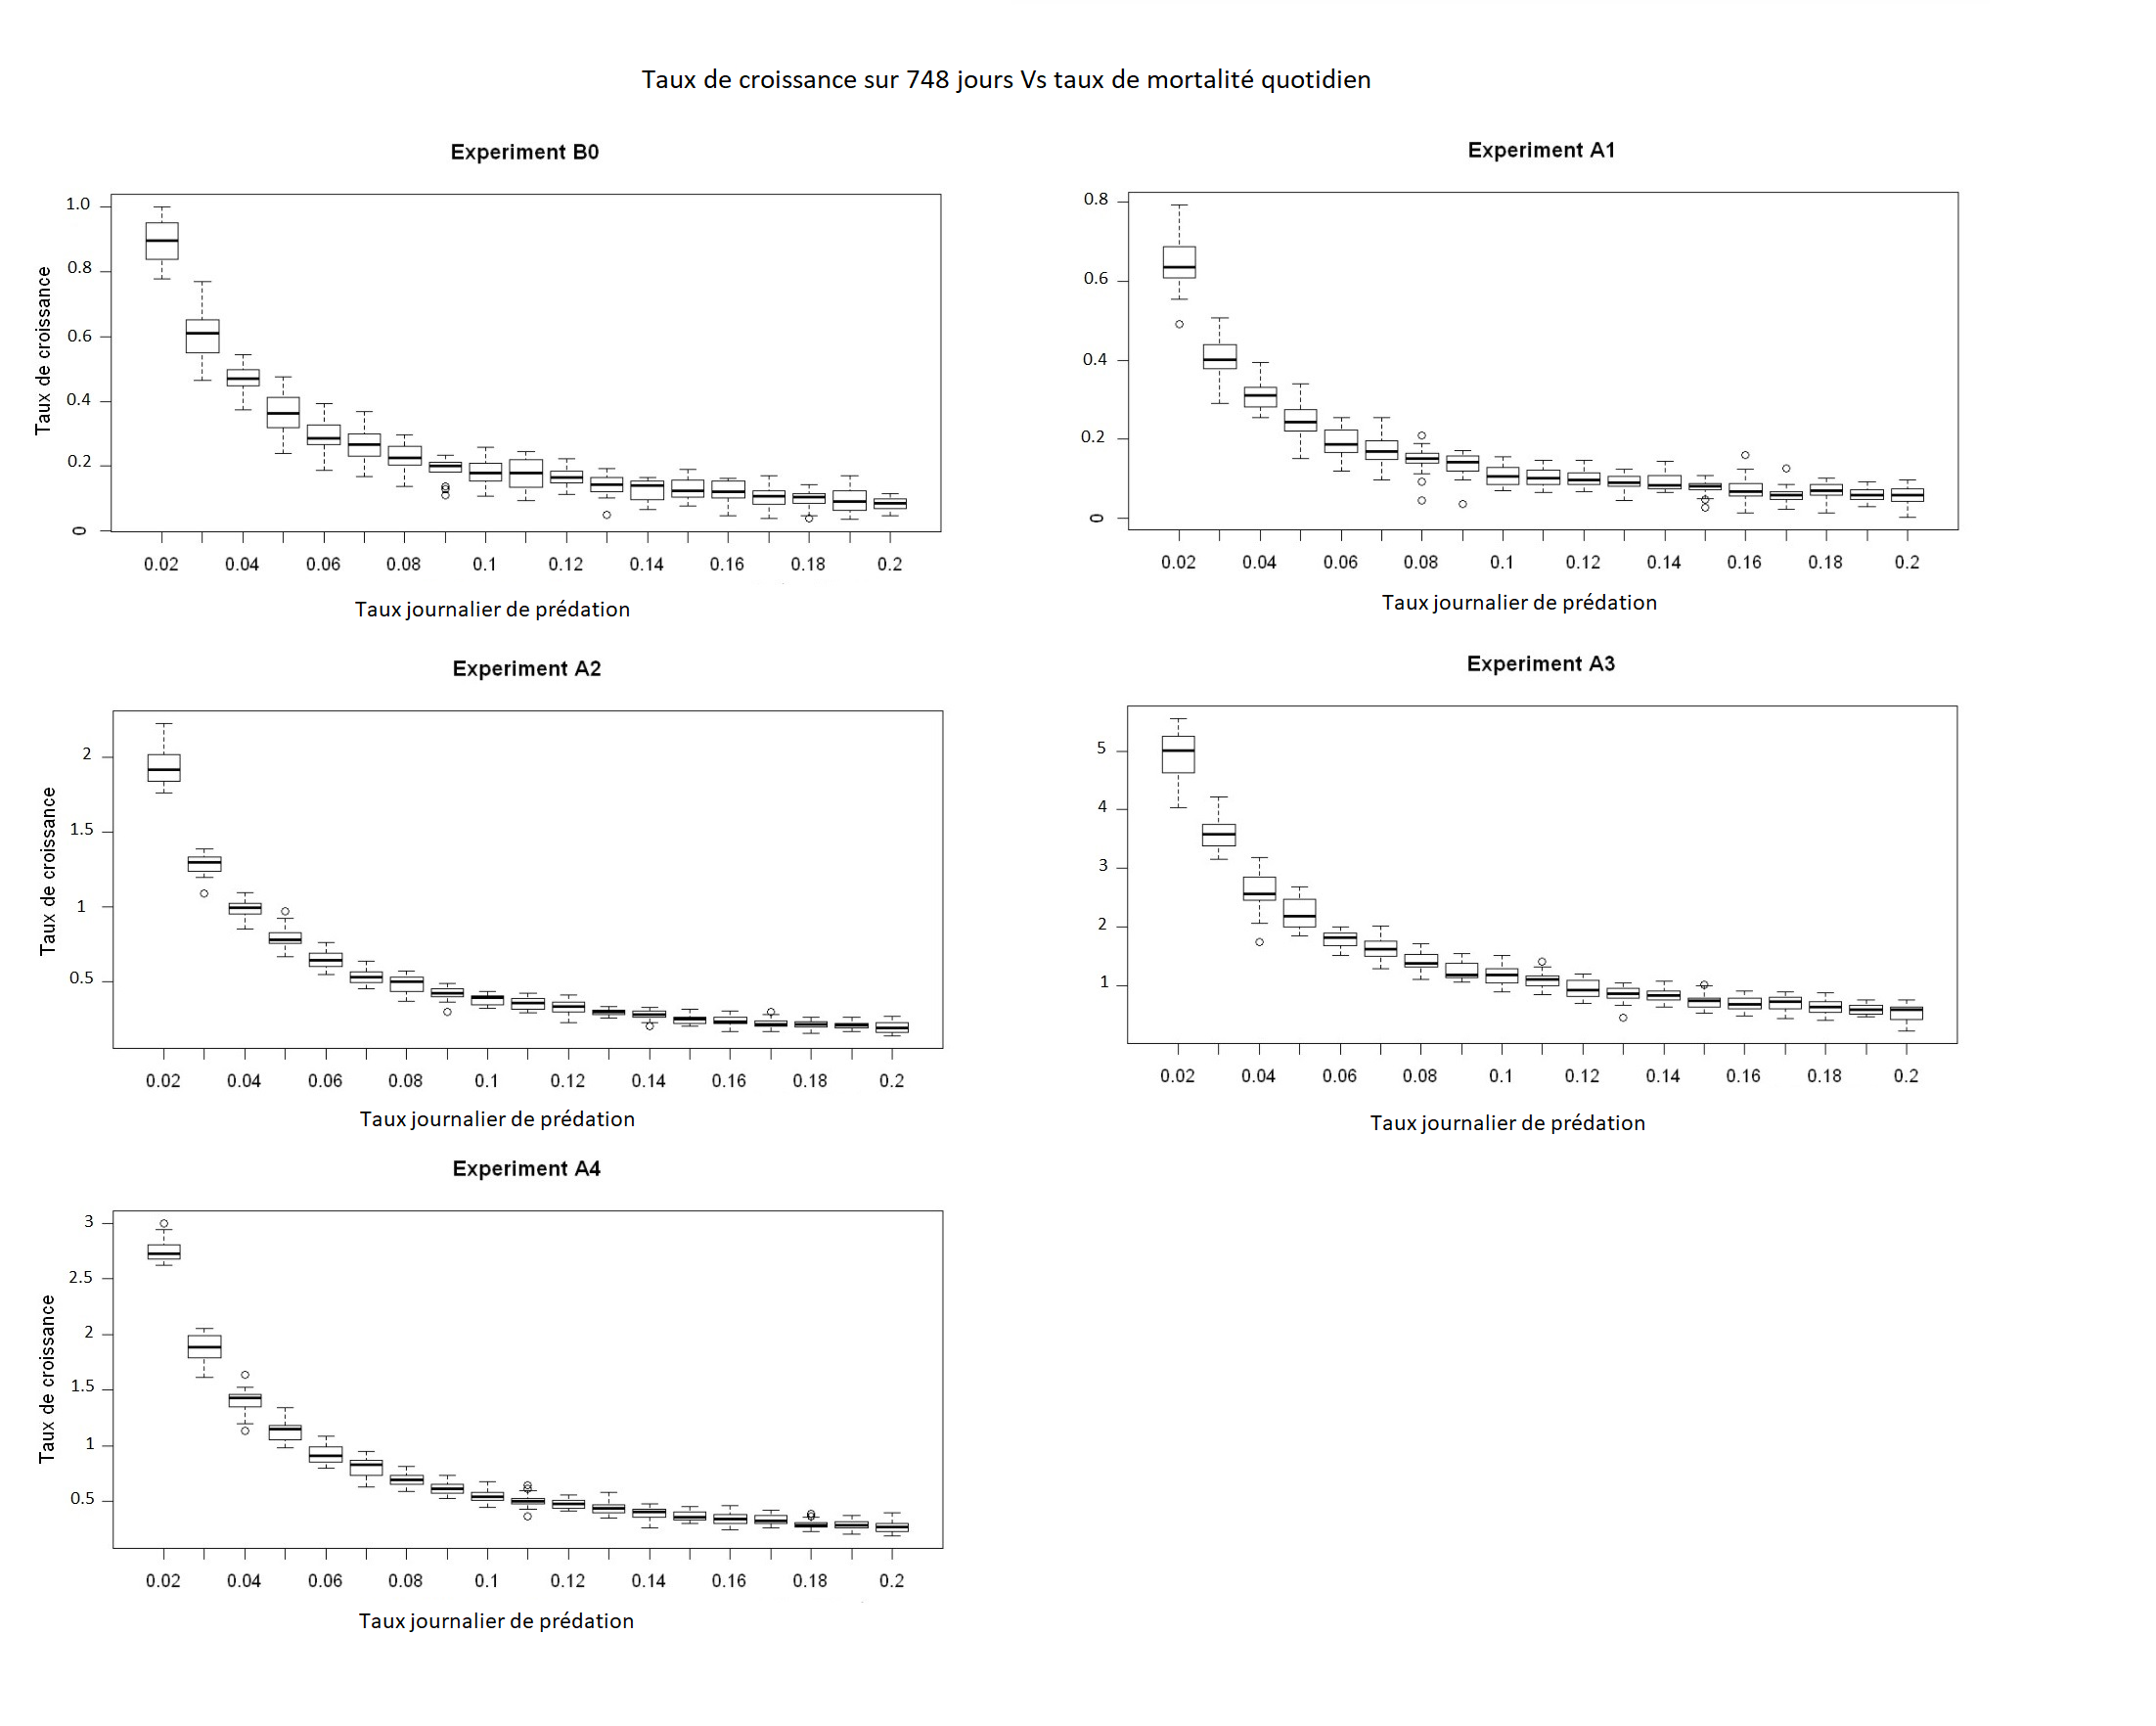
\includegraphics[width=17cm]{tauxcroissance}
	\captionof{figure}{\label{tauxcrs} Analyse de la sensibilité du modèle COSMOS aux paramètres écologiques des parcelles  les plus influents, en se concentrant sur le  paramètre principal de la distribution des taux moyens de régulation quotidienne  sur la parcelle d’expérience B0. Une gamme de valeurs a été testée pour le paramètre, les autres paramètres étant maintenus constants. Le résultat de 20 exécutions a été calculé dans un boxplot.}
\end{figure}
\noindent{Sous l'hypoyhèse des taux de prédation pouvant aller jusqu'à 70 \% (\cite{perfecto1998deployment}) au bout de deux ans dans des champs diversifiés, il a été choisi, en se basant sur les boxplot, comme taux de prédation quotidien 0.03}
\subsubsection{Résultat}
\noindent{La croissance de la population des ravageurs a été affectée par l'organisation spatiale dans leur environnement proche (Fig. \ref{patterns}). Cependant, les effets de l'organisation spatiale diffèrent selon la durée de vie des charançons. On observe une réduction subite de la population des charançons (0,2 ±  0,1) entre le 1er et le 100ième jour pour les patterns d’expérience (ExperimentB0 et ExpérimentA1). La population croit après les 100 jours mais est régulée par l’activité favorable des cultures associées. Par contre pour les patterns d’expérience ExperimentA2, ExperimentA3 et ExperimentA4 (Fig. \ref{patterns}) la population connait une même baisse entre les 100 premiers jours mais croit de manière presque linéaire après jusqu’aux 748ème jours. Comme résultat, la configuration spatiale (ExperimentB0 et ExperimentA1) où les plantes de bananiers sont intercalées avec les plantes de maïs favorise une meilleure gestion de ravageurs par des prédateurs généralistes. La régulation observée durant les 100 premier jours pour toutes les configuration est due à la densité des ravageurs au début du modèle, ce qui favorise l'efficacité de l'activité des ravageurs (\cite{davies2012introduction}).}

\begin{figure}
	\centering
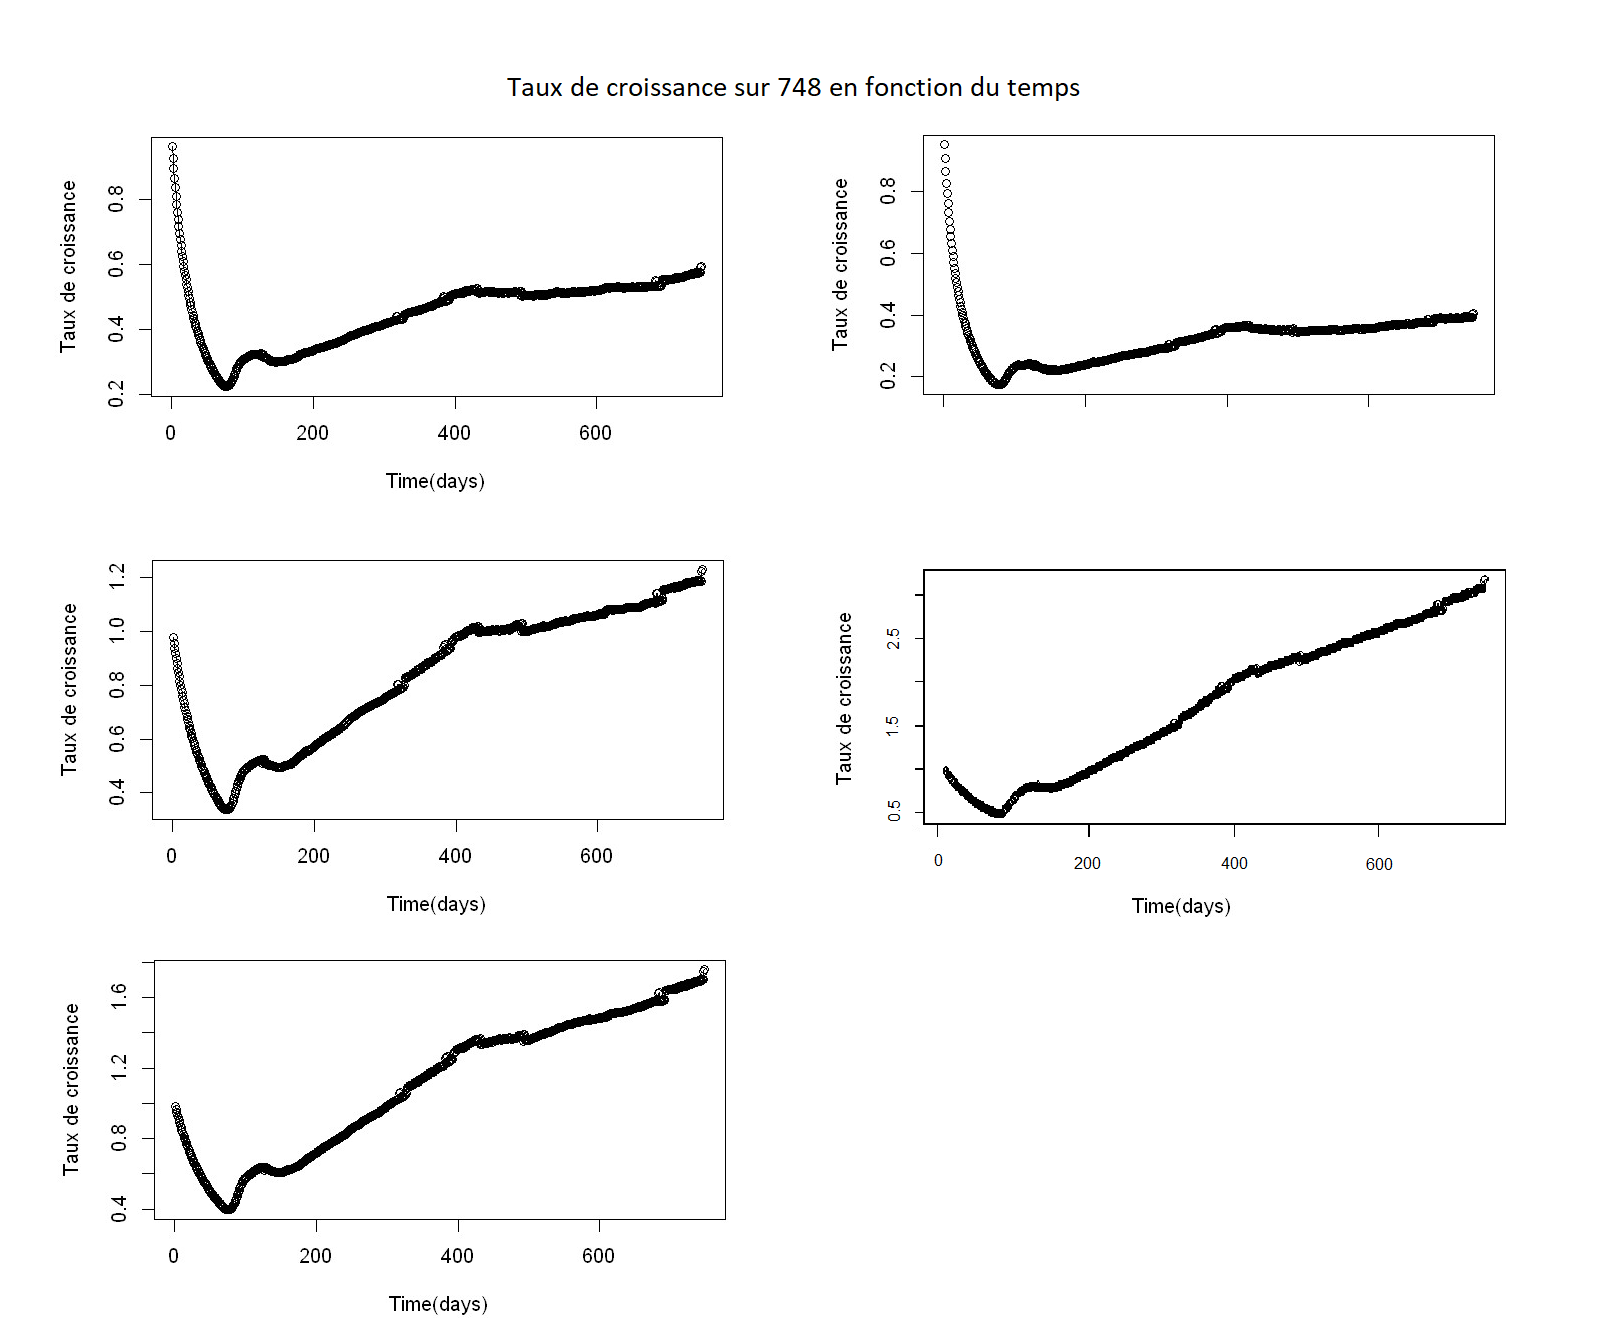
\includegraphics[width=17cm]{croissancetemps}
\captionof{figure}{\label{tauxcrs} Simulation de la distribution du taux de croissance des ravageurs en fonction du temps.}
\end{figure}

\subsubsection{Discussion}
\noindent{En partant d'un modèle spatialement explicite pour une prédation dans des champs de bananiers avec cultures associées, nous avons montré que le taux de croissance de la population des ravageurs peut-être affecté par la configuration spatiale de la parcelle. En ne prenant pas en compte l’intervalle de plantation des cultures, le cycle de maïs  et la mobilité des prédateurs, ce modèle nous a permis de mieux comprendre la régulation des ravageurs causée par la présence des cultures associées (maïs).

Le modèle omet certains comportements ou interactions complexes, tels que le mouvement du prédateur dépendant de la densité ou la capacité du prédateur à évaluer la qualité de l'habitat à distance, qui pourraient influencer la recherche de nourriture, le cycle de maïs qui varie selon le temps et qui pourrait ralenti la régulation pendant la récolte,  Ces omissions peuvent donc réduire le pouvoir prédictif du modèle. Néanmoins, le modèle est une première étape et peut être modifié à l'avenir par l'ajout de complexité en fonction de l'espèce et du système considérés.

Notre modèle ne représente pas les prédateurs ou le cycle des maïs. Notre approche diffère de celle de \cite{collard2018spatial} qui représente la dynamique des \textit{E. caraibea} en omettant les charançons. Cependant, l'inclusion des prédateurs généralistes nécessite généralement des hypothèses concernant la dynamique des prédateurs et les interactions avec les ravageurs, ce qui peut rendre les résultats moins généralisables ou conduire à une propagation des erreurs si les hypothèses sont inexactes. Ceci suggère donc une question qui est de savoir s'il est toujours pertinent d'utiliser la modélisation multi-agent à des questions agroécologiques, à cause de la complexité des systèmes de cultures. Dans l'étude actuelle, l'effet potentiel des prédateurs sur les ravageurs a été évalué par l’hypothèse de distribution des taux de prédation aux pieds des plantes en fonction du voisinage d’habitat favorable. Ces mesures représentent bien l'effet de l'association de maïs sur la régulation du \textit{C. sordidus} si la présence d'un plant de maïs est suffisant pour fixer un taux de prédation journalier au charançons se trouvant aux alentours. Cette hypothèse pourraient être plus améliorées en réalisant des mesures journalières sur une durée de 3 mois minimum avec des méthodes de technologie avancée (observation avec caméra ou par image) et intégrant le cycle de maïs  selon la température. 

En paramétrant le modèle sur des configurations des champs de bananiers et maïs, nous avons constaté que le taux de prédation allait de 0,4 à 0,6 durant la période de simulation pour des configurations bien hétérogènes. Ce taux est, par contre, au dessus de 1 pour des associations regroupées (faible hétérogénéité). Cependant, notre modèle nécessite une validation avant que les résultats puissent être reliés quantitativement aux caractéristiques de l'effet de la configuration spatiale sur le taux de prédation dans les cultures de bananier associées au maïs. Nous interprétons donc nos résultats de manière qualitative. Aussi, les effets secondaires doivent être pris en compte avant que les agriculteurs ne soient invités à mettre en œuvre une organisation spatiale donnée, comme la capacité d’une culture associée à habiter les prédateurs spécifiques pouvant éliminer les parasites ou le potentiel de concurrence entre les plantes cultivées et non cultivées, comme déjà étudié dans les bananeraies (\cite{poeydebat2016balancing},
\cite{collard2018spatial}). 
}

\noindent{}

\subsubsection{Conclusion}
\noindent{Les résultats de la présente étude démontrent que la diversité des cultures affecte fortement le contrôle biologique des ravageurs. Nous avons constaté que l’effet des prédateurs par parcelle est fortement affecté par la configuration spatiale. Nous remarquons également que, plus le champ est bien hétérogène en bananiers et maïs, plus la prédation est efficace. Par contre, une association bananiers et maïs par groupe (bananiers à part et maïs) n'influence pas sur la population du charançon à long terme.  Dans l'ensemble, nos résultats suggèrent que l'organisation spatiale des cultures associées est un outil qui peut être utilisé par les agriculteurs pour améliorer la lutte biologique des ravageurs\\
Compte tenu des processus, des échelles et des périodes pris en compte dans le modèle, et de l'utilisation d'hypothèses communément acceptées sur le taux de prédation, nous pensons que les résultats de l'étude peuvent être considérés comme assez robustes pour une diversité de cultures associées à moins que ces cultures se comportent très différemment dans leur réponse à l’ennemi naturel qu’elles fournissent
}
\subsection{Conclusion générale}
\noindent{La première partie de stage a permis de prendre en compte les interactions de la population des ravageurs avec leur environnement à travers une analyse statistique des données relevées sur le terrain. Dans la seconde partie, des résultats obtenus à partir d’une analyse (GLMM) ont pu être intégrés dans un modèle simulatoire.

Les analyses statistiques ont permis ainsi d’estimer le paramètre d’étude de notre modèle biologique et qui sera par la suite intégré dans les règles de décisions comportementales de l’agent biologique. Une fois le modèle validé à partir de données expérimentales, il pourra être utilisé pour expliqué les différents comportements de la population des ravageurs observés à l'échelle de la parcelle.}


%% Chapter 3

\chapter{Matériel et Méthodes} % Main chapter title
\label{Chapter3} % For referencing the chapter elsewhere, use \ref{Chapter1}
\minitoclt

%----------------------------------------------------------------------------------------

\section{Matériels}
Welcome to this \LaTeX{} Thesis Template, a beautiful and easy to use template for writing a thesis using the \LaTeX{} typesetting system.

If you are writing a thesis (or will be in the future) and its subject is technical or mathematical (though it doesn't have to be), then creating it in \LaTeX{} is highly recommended as a way to make sure you can just get down to the essential writing without having to worry over formatting or wasting time arguing with your word processor.

\LaTeX{} is easily able to professionally typeset documents that run to hundreds or thousands of pages long. With simple mark-up commands, it automatically sets out the table of contents, margins, page headers and footers and keeps the formatting consistent and beautiful. One of its main strengths is the way it can easily typeset mathematics, even \emph{heavy} mathematics. Even if those equations are the most horribly twisted and most difficult mathematical problems that can only be solved on a super-computer, you can at least count on \LaTeX{} to make them look stunning.

%----------------------------------------------------------------------------------------

\section{Méthodes}

\LaTeX{} is not a \textsc{wysiwyg} (What You See is What You Get) program, unlike word processors such as Microsoft Word or Apple's Pages. Instead, a document written for \LaTeX{} is actually a simple, plain text file that contains \emph{no formatting}. You tell \LaTeX{} how you want the formatting in the finished document by writing in simple commands amongst the text, for example, if I want to use \emph{italic text for emphasis}, I write the \verb|\emph{text}| command and put the text I want in italics in between the curly braces. This means that \LaTeX{} is a \enquote{mark-up} language, very much like HTML.


%% Chapter 4

\chapter{Résultats et Discussion} % Main chapter title
\label{Chapter4} % For referencing the chapter elsewhere, use \ref{Chapter1}
\minitoclt

%----------------------------------------------------------------------------------------

\section{Trait de côte et Erosion côtière}
Welcome to this \LaTeX{} Thesis Template, a beautiful and easy to use template for writing a thesis using the \LaTeX{} typesetting system.

If you are writing a thesis (or will be in the future) and its subject is technical or mathematical (though it doesn't have to be), then creating it in \LaTeX{} is highly recommended as a way to make sure you can just get down to the essential writing without having to worry over formatting or wasting time arguing with your word processor.

\LaTeX{} is easily able to professionally typeset documents that run to hundreds or thousands of pages long. With simple mark-up commands, it automatically sets out the table of contents, margins, page headers and footers and keeps the formatting consistent and beautiful. One of its main strengths is the way it can easily typeset mathematics, even \emph{heavy} mathematics. Even if those equations are the most horribly twisted and most difficult mathematical problems that can only be solved on a super-computer, you can at least count on \LaTeX{} to make them look stunning.

%----------------------------------------------------------------------------------------

\section{Etat de l’art}

\LaTeX{} is not a \textsc{wysiwyg} (What You See is What You Get) program, unlike word processors such as Microsoft Word or Apple's Pages. Instead, a document written for \LaTeX{} is actually a simple, plain text file that contains \emph{no formatting}. You tell \LaTeX{} how you want the formatting in the finished document by writing in simple commands amongst the text, for example, if I want to use \emph{italic text for emphasis}, I write the \verb|\emph{text}| command and put the text I want in italics in between the curly braces. This means that \LaTeX{} is a \enquote{mark-up} language, very much like HTML.


%% Chapter 1

\chapter{Généralités sur la prédiction de l’évolution du trait de côte} % Main chapter title
\label{Chapter5} % For referencing the chapter elsewhere, use \ref{Chapter1}
\minitoclt

%----------------------------------------------------------------------------------------

\section{Trait de côte et Erosion côtière}
Welcome to this \LaTeX{} Thesis Template, a beautiful and easy to use template for writing a thesis using the \LaTeX{} typesetting system.

If you are writing a thesis (or will be in the future) and its subject is technical or mathematical (though it doesn't have to be), then creating it in \LaTeX{} is highly recommended as a way to make sure you can just get down to the essential writing without having to worry over formatting or wasting time arguing with your word processor.

\LaTeX{} is easily able to professionally typeset documents that run to hundreds or thousands of pages long. With simple mark-up commands, it automatically sets out the table of contents, margins, page headers and footers and keeps the formatting consistent and beautiful. One of its main strengths is the way it can easily typeset mathematics, even \emph{heavy} mathematics. Even if those equations are the most horribly twisted and most difficult mathematical problems that can only be solved on a super-computer, you can at least count on \LaTeX{} to make them look stunning.

%----------------------------------------------------------------------------------------

\section{Etat de l’art}

\LaTeX{} is not a \textsc{wysiwyg} (What You See is What You Get) program, unlike word processors such as Microsoft Word or Apple's Pages. Instead, a document written for \LaTeX{} is actually a simple, plain text file that contains \emph{no formatting}. You tell \LaTeX{} how you want the formatting in the finished document by writing in simple commands amongst the text, for example, if I want to use \emph{italic text for emphasis}, I write the \verb|\emph{text}| command and put the text I want in italics in between the curly braces. This means that \LaTeX{} is a \enquote{mark-up} language, very much like HTML.


%% Conclusion

\chapter*{Conclusion Générale et Perspectives} % Main chapter title
\label{conclusion} % For referencing the chapter elsewhere, use \ref{Chapter1}
\addcontentsline{toc}{chapter}{Conclusion}
%\minitoclt

%----------------------------------------------------------------------------------------

Welcome to this \LaTeX{} Thesis Template, a beautiful and easy to use template for writing a thesis using the \LaTeX{} typesetting system.

If you are writing a thesis (or will be in the future) and its subject is technical or mathematical (though it doesn't have to be), then creating it in \LaTeX{} is highly recommended as a way to make sure you can just get down to the essential writing without having to worry over formatting or wasting time arguing with your word processor.

\LaTeX{} is easily able to professionally typeset documents that run to hundreds or thousands of pages long. With simple mark-up commands, it automatically sets out the table of contents, margins, page headers and footers and keeps the formatting consistent and beautiful. One of its main strengths is the way it can easily typeset mathematics, even \emph{heavy} mathematics. Even if those equations are the most horribly twisted and most difficult mathematical problems that can only be solved on a super-computer, you can at least count on \LaTeX{} to make them look stunning.



%----------------------------------------------------------------------------------------
%	THESIS CONTENT - APPENDICES
%----------------------------------------------------------------------------------------

\appendix % Cue to tell LaTeX that the following "chapters" are Appendices

% Include the appendices of the thesis as separate files from the Appendices folder
% Uncomment the lines as you write the Appendices

%% Appendix A

\chapter{Annexes} % Main appendix title
\label{AppendixA} % For referencing this appendix elsewhere, use \ref{AppendixA}

\section{How do I change the colors of links?}

The color of links can be changed to your liking using:

{\small\verb!\hypersetup{urlcolor=red}!}, or

{\small\verb!\hypersetup{citecolor=green}!}, or

{\small\verb!\hypersetup{allcolor=blue}!}.

\noindent If you want to completely hide the links, you can use:

{\small\verb!\hypersetup{allcolors=.}!}, or even better:

{\small\verb!\hypersetup{hidelinks}!}.

\noindent If you want to have obvious links in the PDF but not the printed text, use:

{\small\verb!\hypersetup{colorlinks=false}!}.

%\include{Appendices/AppendixB}
%\include{Appendices/AppendixC}

%----------------------------------------------------------------------------------------
%	BIBLIOGRAPHY
%----------------------------------------------------------------------------------------

\printbibliography
%----------------------------------------------------------------------------------------
\end{document}